\documentclass[%
%draft,
11pt,%
twoside,%
titlepage,%
swissgerman,%
headsepline%
]{scrartcl}

\usepackage{lastpage}
\usepackage{amsthm}
\usepackage{amssymb}
\usepackage{geometry}
\usepackage{graphicx}
\usepackage[dvipsnames]{xcolor}
\usepackage[utf8]{inputenc}
\usepackage[swissgerman]{babel}
\usepackage{lscape}
\usepackage[framemethod=TikZ]{mdframed}
\usepackage[most]{tcolorbox}
\usepackage{enumerate}
\usepackage{units}
\usepackage{nicefrac}
\usepackage{pgf,tikz}
\usepackage{tikz-3dplot}
\usepackage{tkz-euclide}
\usetikzlibrary{arrows}
\usetikzlibrary{arrows.meta}
\usetikzlibrary{patterns}
\usetikzlibrary{positioning}
\usetikzlibrary{shadows}
\usetikzlibrary{quotes, angles}
\usepackage{colortbl}
\usepackage{hhline}
\usepackage{multirow}
\usepackage[extendedchars]{grffile}
\usepackage{caption}
\usepackage{multicol,calc}
\usepackage{blindtext}
\usepackage{pdfpages}
\usepackage{hyperref}
\usepackage{framed}

\usepackage{marginnote}
\usepackage{qrcode}
<<<<<<< Updated upstream
\qrset{height=9ex}
=======
\qrset{height=7ex}
>>>>>>> Stashed changes

\usepackage{longtable}
\usepackage{listings}
\usepackage{wrapfig}

\usepackage{fontawesome} % Oder FontAwesome, falls du ein Augensymbol aus einer
\newcommand{\faEyeLightGray}{\textcolor{lightgray}{\faEye}} % Custom command for the gray eye icon
\newcommand{\faReturnGray}{\textcolor{gray}{\faMailReply}} % Custom command for the gray eye icon
\usepackage{pifont} % weitere Zeichen

% package für plots mit dem Befehl axes
\usepackage{pgfplots}



% Command, um Tabellen-Spalten anzupassen
\newcommand{\spaltenheight}{\rule{0mm}{3ex}}
\newcommand{\spaltenwidth}{\rule{3cm}{0mm}}
\newcommand{\spaltensep}{\\[1ex]}
%\arrayrulecolor{darkgreen}
\doublerulesepcolor{white}

% colors
\definecolor{lightyellow}{rgb}{1,1,0.8}
\definecolor{Gray}{gray}{0.9}
\definecolor{lightgray}{rgb}{0.7, 0.7, 0.7}
\definecolor{darkblue}{rgb}{0,0,0.55}
\definecolor{firebrick}{rgb}{0.7,0.13,0.13}
\definecolor{seagreen}{rgb}{0.18,0.55,0.34}
\definecolor{emerald}{HTML}{50C878} % color of Definition
\definecolor{whitesmoke}{HTML}{F5F5F5} % background for environments
\definecolor{myblizzardblue}{HTML}{87CEEB} % color of Satz

% Für Definitionen im Fliesstext
\newcommand{\definition}[1]{\colorbox{emerald}{#1}}
% Für Regeln im Fliesstext
\newcommand{\regel}[1]{\colorbox{myblizzardblue}{#1}}
% Für Merke/Achtungs im Fliesstext
\newcommand{\merke}[1]{\colorbox{firebrick}{#1}}
% Geogebra-Link
\newcommand{\geogebralink}{\href{https://www.geogebra.org/calculator}{\texttt{geogebra.org}}}

% Umgebungen
\theoremstyle{definition}
    \newtheorem{bsp}{Beispiel}[subsection] % Beispiele
    \newtheorem{bem}{Bemerkung}[subsection] % Bemerkungen
\theoremstyle{plain}
    \newtheorem{thm}{Theorem} % Theorem [subsection]
    \newtheorem{satz}{Satz} % Satz [subsection]

% Umgebung lsg mit dynamischer Referenzierung und Label
\newcommand{\concatueb}[1]{ueb:#1}% Definition für concatueb
\newcommand{\concatlsg}[1]{lsg:#1}% Definition für concatlsg

\newcounter{uebcounter}[section]
\renewcommand{\theuebcounter}{\thesection.\arabic{uebcounter}}  % Zählerformat: Abschnitt.Übung

\newenvironment{lsg}[1]{%
<<<<<<< Updated upstream
    \par\noindent\textbf{Notizen zu Übung \theuebcounter\label{\concatlsg{#1}}}
=======
    \par\noindent\textbf{Notizen zu Übung \ref{\concatueb{#1}}}\label{\concatlsg{#1}}
>>>>>>> Stashed changes
    \hfill\hyperref[\concatueb{#1}]{\faReturnGray}\par % Hyperref-Button zurück zur Übung
}{%
    \par%
}

\newenvironment{uebenv}[1]{%
    \refstepcounter{uebcounter}
    \par\noindent\textbf{Übung \theuebcounter.}%
    \label{\concatueb{#1}}\hfill\hyperref[\concatlsg{#1}]{\faEyeLightGray}\par
}{%
    \par
}

% Umgebung für Definitionen
\newcounter{deff}[section]\setcounter{deff}{0}
\renewcommand{\thedeff}{\arabic{section}.\arabic{deff}}

\newenvironment{cdef}[1][]{%
    \refstepcounter{deff} 
    \ifstrempty{#1}%
    % if condition (without title)
    {\mdfsetup{%
        frametitle={%
            \tikz[baseline=(current bounding box.east),outer sep=0pt]
            \node[anchor=east,rectangle,fill=emerald]
            {\strut Definition~\thedeff};}
        }%
    % else condition (with title)
    }{\mdfsetup{%
        frametitle={%
            \tikz[baseline=(current bounding box.east),outer sep=0pt]
            \node[anchor=east,rectangle,fill=emerald]
            {\strut Definition~\thedeff:~#1};}%
        }%
    }%
% for both conditions
    \mdfsetup{%
        innertopmargin=10pt,linecolor=emerald,%
        backgroundcolor=whitesmoke,%
        linewidth=2pt,topline=true,%
        frametitleaboveskip=\dimexpr-\ht\strutbox\relax%
    } 
\begin{mdframed}[]\relax}{%
\end{mdframed}}

% Farbig umrahmte Umgebung Satz
\newcounter{satzz}[section]\setcounter{satzz}{0}
\renewcommand{\thesatz}{\arabic{section}.\arabic{satzz}}

\newenvironment{csatz}[1][]{%
    \refstepcounter{satzz}
 
    \ifstrempty{#1}%
    % if condition (without title)
    {\mdfsetup{%
        frametitle={%
            \tikz[baseline=(current bounding box.east),outer sep=0pt]
            \node[anchor=east,rectangle,fill=myblizzardblue]
            {\strut Satz~\thesatz};}
        }%
    % else condition (with title)
    }{\mdfsetup{%
        frametitle={%
            \tikz[baseline=(current bounding box.east),outer sep=0pt]
            \node[anchor=east,rectangle,fill=myblizzardblue]
            {\strut Satz~\thesatz:~#1};}%
        }%
    }%
% for both conditions
    \mdfsetup{%
        innertopmargin=10pt,linecolor=myblizzardblue,%
        backgroundcolor=whitesmoke,%
        linewidth=2pt,topline=true,%
        frametitleaboveskip=\dimexpr-\ht\strutbox\relax%
    }
\begin{mdframed}[]\relax}{%
\end{mdframed}}

% kein Einzug bei neuem Abschnitt
\setlength{\parindent}{0pt} \setlength{\parskip}{1em}
\pagestyle{headings} % gemachte Einstellungen anwenden


\subject{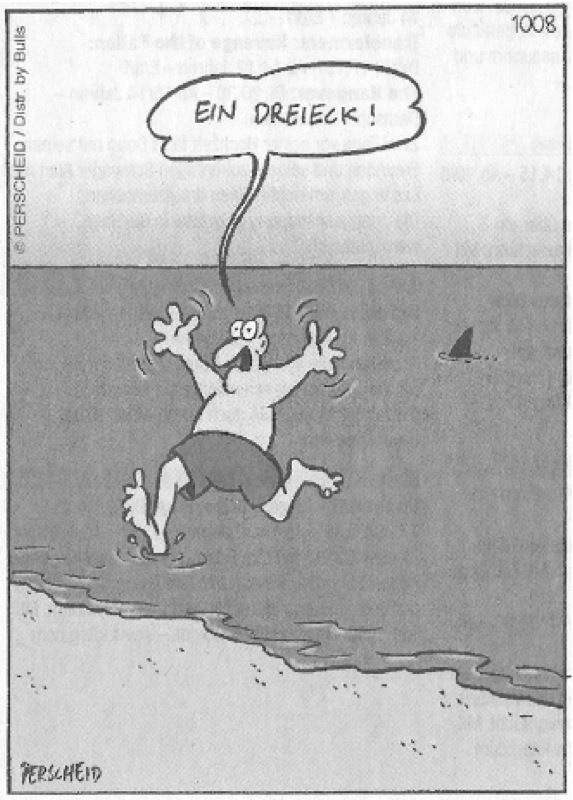
\includegraphics[width=0.618\textwidth]{pictures/dreiecksw.jpg}}
\title{Geometrie}
\subtitle{Rund um Ecken und Kanten}
\author{}
\date{}
\lowertitleback{

\includegraphics[height=1cm]{pictures/gymfmslerbermattlogo.eps}
\hfill%\copyright%
{\begin{tikzpicture}
  % Draw the rounded rectangle and clip the image to it
  \clip [rounded corners=5mm] (0,0) rectangle (1,1); % Adjust dimensions as needed
  \node at (0.5,0.5) {\includegraphics[width=1cm]{pictures/teacher_me_caricatur.png}}; % Adjust width and center image
\end{tikzpicture}}
}

\begin{document}
\maketitle
\tableofcontents
%\thispagestyle{empty}
\cleardoublepage
%\setcounter{page}{1}

\section{Planimetrie}

\subsection{Testfragen Basics}

\begin{uebenv}{testfragen}
    
Welche der folgenden Aussagen sind richtig, welche falsch? Ist die Aussage richtig, dann versuche sie zu begr\"unden. Ist die Aussage falsch, dann gib ein Gegenbeispiel.
\begin{enumerate}
\item Zwei Geraden haben genau einen Schnittpunkt
\item Die Summe eines Winkels $\alpha$ und seines Stufenwinkels betr\"agt $180^\circ $.
\item Die Winkelsumme im Dreieck betr\"agt $180^\circ $
\item Der $90^\circ $-Winkel kann konstruiert werden.
\item Der $15^\circ $-Winkel kann konstruiert werden.
\item Wird hintereinander an zwei verschiedenen Achsen gespiegelt, so erh\"alt man eine Verschiebung.
\item Eine Punktspiegelung entspricht einer Drehung um $180^\circ $.
\item Zwei Dreiecke sind kongruent, wenn sie in drei Seiten \"ubereinstimmen.
\item Die Innenwinkelsumme eines $n$-Ecks berechnet sich nach der Formel
$$2^{n-3}\cdot180^\circ .$$
\item Der Umkreismittelpunkt eines Dreiecks liegt im Innern des Dreiecks.
\item Halbieren sich die Diagonalen im einem Viereck, und besitzt das Viereck mindestens einen rechten Winkel, so handelt es sich um ein Rechteck.
\item Ein Parallelogramm ist ein spezielles Trapez.
\item Ein Rhombus besitzt gleich viele Symmetrieachsen wie ein gleichseitiges Dreieck.
\item Der Fl\"acheninhalt eines rechtwinkligen Dreiecks ($\gamma=90^\circ $) ist
$$A=\frac{ab}{2}$$
\item Die Mittelsenkrechte einer Sehne eines Kreises geht durch den Mittelpunkt des Kreises.
\item Der Kreisbogen eines Kreises ist proportional zu seinem Zentriwinkel.
\item Der Fl\"acheninhalt eines Kreises ist proportional zu seinem Radius.
\item Die Mittellinie eines Trapezes ABCD mit den parallelen Seiten $a$ und $c$ hat die L\"ange
$$m=\frac{a+c}{2}$$
\item Die Peripheriewinkel \"uber einer Sehne sind alle gleich gross und halb so gross wie ihr Zentriwinkel.
\item Der Satz des Thales ist eine direkte Folgerung aus der oben genannten Feststellung.
\end{enumerate}

\end{uebenv}

\subsection{Konstruieren}
Man hält grundsätzlich an folgenden Konventionen fest:
\begin{itemize}
\item Konstruktionen sind mit Zirkel und Lineal durchzuf\"uhren.
\item Nicht konstruierbare Winkel misst man mit dem Geo-Dreieck (zB. $20^\circ $)
\item Zu Geometrieaufgaben geh\"oren im Allgemeinen eine Skizze und ein kurzer Kon\-struk\-tions\-bericht.
\end{itemize}

\begin{uebenv}{konstruieredreiecke}
Konstruiere Dreiecke aus folgenden Angaben:

    \begin{enumerate}[a)]
      %\item $a=\unit[6]{cm}$, $b=\unit[8]{cm}$, $c=\unit[7]{cm}$
      \item $c=\unit[5]{cm}$, $a=\unit[8]{cm}$, $\beta=40^\circ $
      \item $a=\unit[8]{cm}$, $\alpha=50^\circ $, $\beta=70^\circ $
      \item $a=\unit[5]{cm}$, $b=\unit[8]{cm}$, $\alpha=55^\circ $
      \item $a=\unit[7]{cm}$, $b=\unit[8]{cm}$, $\alpha=55^\circ $
      \item $a=\unit[9]{cm}$, $b=\unit[8]{cm}$, $\alpha=55^\circ $
    \end{enumerate}
\end{uebenv}

\subsection{Winkel am Kreis}
Es gilt bekanntlich folgender

\begin{csatz}[Peripheriewinkelsatz]
Der Peripheriewinkel \"uber einer Sehne $\overline{AB}$ ist halb so gross wie der zugeh\"orige Zentriwinkel.
\end{csatz}

\begin{proof}
Siehe \"Ubungen.
\end{proof}

\begin{bem}
Aus dem Beweis folgt direkt, dass alle Peripheriewinkel \"uber gleichem Bogen gleich gross sind.
\end{bem}

\begin{figure}
\begin{center}
<<<<<<< Updated upstream
\definecolor{qqwuqq}{rgb}{0,0.39,0}
\definecolor{uququq}{rgb}{0.25,0.25,0.25}
\scalebox{0.618}{
\begin{tikzpicture}[line cap=round,line join=round,>=triangle 45,x=1.0cm,y=1.0cm]
\clip(-4.52,-4.38) rectangle (4.92,4.3);
\draw [shift={(2.41,3.19)},line width=1.6pt,color=qqwuqq,fill=qqwuqq,fill opacity=0.1] (0,0) -- (-142.7:0.8) arc (-142.7:-87.97:0.8) -- cycle;
\draw [shift={(0,0)},line width=1.6pt,color=qqwuqq,fill=qqwuqq,fill opacity=0.1] (0,0) -- (-158.3:0.8) arc (-158.3:-48.84:0.8) -- cycle;
=======


\scalebox{0.618}{
\begin{tikzpicture}[line cap=round,line join=round,>=triangle 45,x=1.0cm,y=1.0cm]
\clip(-4.52,-4.38) rectangle (4.92,4.3);
\draw [shift={(2.41,3.19)},line width=1.6pt,color=ForestGreen,fill=ForestGreen,fill opacity=0.1] (0,0) -- (-142.7:0.8) arc (-142.7:-87.97:0.8) -- cycle;
\draw [shift={(0,0)},line width=1.6pt,color=ForestGreen,fill=ForestGreen,fill opacity=0.1] (0,0) -- (-158.3:0.8) arc (-158.3:-48.84:0.8) -- cycle;
>>>>>>> Stashed changes
\draw [line width=2pt] (0,0) circle (4cm);
\draw [line width=1.6pt] (-3.72,-1.48)-- (2.63,-3.01);
\draw [line width=1.6pt] (-3.72,-1.48)-- (2.41,3.19);
\draw [line width=1.6pt] (2.63,-3.01)-- (2.41,3.19);
\draw [line width=1.6pt] (0,0)-- (-3.72,-1.48);
\draw [line width=1.6pt] (0,0)-- (2.63,-3.01);
\begin{scriptsize}
<<<<<<< Updated upstream
\fill [color=uququq] (0,0) circle (1.5pt);
\draw[color=uququq] (0.18,0.26) node {$M$};
=======
\fill [color=Gray] (0,0) circle (1.5pt);
\draw[color=Gray] (0.18,0.26) node {$M$};
>>>>>>> Stashed changes
\fill [color=black] (-3.72,-1.48) circle (1.5pt);
\draw[color=black] (-4.08,-1.48) node {$A$};
\fill [color=black] (2.63,-3.01) circle (1.5pt);
\draw[color=black] (2.68,-3.36) node {$B$};
\fill [color=black] (2.41,3.19) circle (1.5pt);
\draw[color=black] (2.58,3.46) node {$C$};
\end{scriptsize}
\end{tikzpicture}
}
\end{center}
\caption{Peripheriewinkelsatz}
\end{figure}

\begin{uebenv}{epsilonimkreis}
Berechne den Winkel $\epsilon$:
\begin{center}
<<<<<<< Updated upstream
\definecolor{qqwuqq}{rgb}{0,0.39,0}
\scalebox{0.618}{
\begin{tikzpicture}[line cap=round,line join=round,>=triangle 45,x=1.0cm,y=1.0cm]
\clip(-4.3,-4.04) rectangle (7.26,6.3);
\draw [shift={(165.88,139.34)},line width=1.6pt,color=qqwuqq] (0,0) -- (-161.06:1) arc (-161.06:-118.88:1) -- cycle;
\draw [shift={(-2.56,0.36)},line width=1.6pt,color=qqwuqq] (0,0) -- (-19.63:1) arc (-19.63:54.08:1) -- cycle;
=======

\scalebox{0.618}{
\begin{tikzpicture}[line cap=round,line join=round,>=triangle 45,x=1.0cm,y=1.0cm]
\clip(-4.3,-4.04) rectangle (7.26,6.3);
\draw [shift={(165.88,139.34)},line width=1.6pt,color=ForestGreen] (0,0) -- (-161.06:1) arc (-161.06:-118.88:1) -- cycle;
\draw [shift={(-2.56,0.36)},line width=1.6pt,color=ForestGreen] (0,0) -- (-19.63:1) arc (-19.63:54.08:1) -- cycle;
>>>>>>> Stashed changes
\draw [line width=1.6pt] (0,0) circle (2.58cm);
\draw [line width=1.6pt,domain=-4.3:7.26] plot(\x,{(-17.32-2.17*\x)/-6.34});
\draw [line width=1.6pt,domain=-4.3:7.26] plot(\x,{(--17.32-5.87*\x)/-3.24});
\draw [line width=1.6pt] (-1.14,2.32)-- (-2.56,0.36);
\draw [line width=1.6pt] (-2.56,0.36)-- (2.21,-1.34);
\draw (4.86,4.4) node[anchor=north west] {$\epsilon$};
\draw (-2.2,0.75) node[anchor=north west] {$2\epsilon$};
\end{tikzpicture}
}
\end{center}
\end{uebenv}

\begin{uebenv}{stern}
Berechne den Winkel $\epsilon$:
\begin{center}
<<<<<<< Updated upstream
\definecolor{qqwuqq}{rgb}{0,0.39,0}
\definecolor{xdxdff}{rgb}{0.49,0.49,1}
\definecolor{uququq}{rgb}{0.25,0.25,0.25}
\scalebox{1.4}{
\begin{tikzpicture}[line cap=round,line join=round,>=triangle 45,x=1.0cm,y=1.0cm]
\clip(-1.72,-1.34) rectangle (4.78,5.06);
\draw [shift={(3,0)},line width=1.2pt,color=qqwuqq] (0,0) -- (108:1) arc (108:144:1) -- cycle;
=======



\scalebox{1.4}{
\begin{tikzpicture}[line cap=round,line join=round,>=triangle 45,x=1.0cm,y=1.0cm]
\clip(-1.72,-1.34) rectangle (4.78,5.06);
\draw [shift={(3,0)},line width=1.2pt,color=ForestGreen] (0,0) -- (108:1) arc (108:144:1) -- cycle;
>>>>>>> Stashed changes
\draw [line width=2pt] (1.5,2.06) circle (2.55cm);
\draw [line width=1.6pt] (1.5,4.62)-- (0,0);
\draw [line width=1.6pt] (0,0)-- (3.93,2.85);
\draw [line width=1.6pt] (3.93,2.85)-- (-0.93,2.85);
\draw [line width=1.6pt] (-0.93,2.85)-- (3,0);
\draw [line width=1.6pt] (3,0)-- (1.5,4.62);
\draw (-3,5.24) node[anchor=north west] {$\epsilon$};
\draw (2.48,0.7) node[anchor=north west] {$\epsilon$};
\draw (-0.48,4.74) node[anchor=north west] {$b$};
\draw (-1.28,1.28) node[anchor=north west] {b};
\draw (4.14,1.32) node[anchor=north west] {b};
\draw (3.28,4.52) node[anchor=north west] {b};
\draw (1.44,-0.66) node[anchor=north west] {b};
\begin{scriptsize}
<<<<<<< Updated upstream
\fill [color=uququq] (0,0) circle (1.5pt);
\fill [color=xdxdff] (3,0) circle (1.5pt);
\fill [color=uququq] (3.93,2.85) circle (1.5pt);
\fill [color=uququq] (1.5,4.62) circle (1.5pt);
\fill [color=uququq] (-0.93,2.85) circle (1.5pt);
=======
\fill [color=Gray] (0,0) circle (1.5pt);
\fill [color=RoyalBlue] (3,0) circle (1.5pt);
\fill [color=Gray] (3.93,2.85) circle (1.5pt);
\fill [color=Gray] (1.5,4.62) circle (1.5pt);
\fill [color=Gray] (-0.93,2.85) circle (1.5pt);
>>>>>>> Stashed changes
\end{scriptsize}
\end{tikzpicture}
}
\end{center}
\end{uebenv}

\begin{uebenv}{seltsamesdreieck}
Berechne den Winkel $\epsilon$:
\begin{center}
<<<<<<< Updated upstream
\definecolor{qqqqff}{rgb}{0,0,1}
\definecolor{qqwuqq}{rgb}{0,0.39,0}
\scalebox{1}{
\begin{tikzpicture}[line cap=round,line join=round,>=triangle 45,x=1.0cm,y=1.0cm]
\clip(-3.4,-3.58) rectangle (6.1,5.54);
\draw [shift={(1.1,5.16)},line width=1.2pt,color=qqwuqq] (0,0) -- (-118.96:1) arc (-118.96:-44.57:1) -- cycle;
\draw [shift={(1.16,1.16)},line width=1.2pt,color=qqwuqq] (0,0) -- (0:0.6) arc (0:90.86:0.6) -- cycle;
=======


\scalebox{1}{
\begin{tikzpicture}[line cap=round,line join=round,>=triangle 45,x=1.0cm,y=1.0cm]
\clip(-3.4,-3.58) rectangle (6.1,5.54);
\draw [shift={(1.1,5.16)},line width=1.2pt,color=ForestGreen] (0,0) -- (-118.96:1) arc (-118.96:-44.57:1) -- cycle;
\draw [shift={(1.16,1.16)},line width=1.2pt,color=ForestGreen] (0,0) -- (0:0.6) arc (0:90.86:0.6) -- cycle;
>>>>>>> Stashed changes
\draw [line width=1.6pt] (1.16,1.16) circle (4cm);
\draw [line width=1.6pt] (1.16,1.16)-- (5.16,1.16);
\draw [line width=1.6pt,dash pattern=on 5pt off 5pt] (1.1,5.16)-- (1.16,1.16);
\draw [shift={(1.24,-2.84)}] plot[domain=1.59:2.64,variable=\t]({1*4*cos(\t r)+0*4*sin(\t r)},{0*4*cos(\t r)+1*4*sin(\t r)});
\draw [line width=1.6pt] (1.1,5.16)-- (-2.26,-0.91);
\draw [line width=1.6pt] (1.1,5.16)-- (5.16,1.16);
\draw [line width=1.6pt,dotted] (1.16,1.16)-- (1.24,-2.84);
\draw [line width=1.6pt] (-2.27,-0.91)-- (5.16,1.12);
\draw (1.14,4.7) node[anchor=north west] {$\epsilon$};
\begin{scriptsize}
<<<<<<< Updated upstream
\fill [color=qqqqff] (1.44,1.4) circle (1.5pt);
=======
\fill [color=darkblue] (1.44,1.4) circle (1.5pt);
>>>>>>> Stashed changes
\end{scriptsize}
\end{tikzpicture}
}
\end{center}
\end{uebenv}

\begin{uebenv}{zweiradien}
Berechne den Winkel $\epsilon$:
\begin{center}
<<<<<<< Updated upstream
\definecolor{qqwuqq}{rgb}{0,0.39,0}
\scalebox{1}{
\begin{tikzpicture}[line cap=round,line join=round,>=triangle 45,x=1.0cm,y=1.0cm]
\clip(-4.38,-1.18) rectangle (5.26,5.02);
\draw [shift={(2.36,3.82)},line width=1.2pt,color=qqwuqq] (0,0) -- (-120.28:1) arc (-120.28:-75.26:1) -- cycle;
=======

\scalebox{1}{
\begin{tikzpicture}[line cap=round,line join=round,>=triangle 45,x=1.0cm,y=1.0cm]
\clip(-4.38,-1.18) rectangle (5.26,5.02);
\draw [shift={(2.36,3.82)},line width=1.2pt,color=ForestGreen] (0,0) -- (-120.28:1) arc (-120.28:-75.26:1) -- cycle;
>>>>>>> Stashed changes
\draw [shift={(0.31,0.05)},line width=1.6pt]  plot[domain=-0.01:3.13,variable=\t]({1*4.29*cos(\t r)+0*4.29*sin(\t r)},{0*4.29*cos(\t r)+1*4.29*sin(\t r)});
\draw [line width=1.6pt] (-3.98,0.1)-- (4.6,0);
\draw [shift={(-3.98,0.1)},line width=1.6pt]  plot[domain=-0.01:0.53,variable=\t]({1*7.34*cos(\t r)+0*7.34*sin(\t r)},{0*7.34*cos(\t r)+1*7.34*sin(\t r)});
\draw [shift={(4.6,0)},line width=1.6pt]  plot[domain=2.1:3.13,variable=\t]({1*4.43*cos(\t r)+0*4.43*sin(\t r)},{0*4.43*cos(\t r)+1*4.43*sin(\t r)});
\draw [line width=1.6pt] (2.36,3.82)-- (3.36,0.01);
\draw [line width=1.6pt] (0.16,0.05)-- (2.36,3.82);
\draw [->,dash pattern=on 2pt off 2pt] (-3.98,0.1) -- (3.12,1.97);
\draw [->,dash pattern=on 2pt off 2pt] (4.6,0) -- (0.78,2.25);
\draw (2,3.3) node[anchor=north west] {$\epsilon$};
\end{tikzpicture}
}
\end{center}
\end{uebenv}

\clearpage

\subsection{Notizen zu den Übungen}

\begin{lsg}{testfragen}
    \begin{enumerate}
        \item \ding{55}, die Geraden können parallel laufen. Dann haben sie keinen oder unendlich viele Schnittpunkte.
        \item \ding{55}, $2\alpha$
        \item \ding{51} für die Innenwinkelsumme. Für einen Beweis betrachte man eine Dreieckseite und ihre Parallele durch die gegenüberliegende Ecke. Die Stufen- und der Zentriwinkel zusammen ergeben $180^\circ$.
        \item \ding{51}, Mittelsenkrechte
        \item \ding{51}, man halbiert einen konstruierten $60^\circ$ Winkel zweimal.
        \item \ding{55}, denn beispielsweise zwei Achsenspiegelungen ($x$- und $y$-Achse) ergeben eine Drehung um $180^\circ$ um den Ursprung.
        \item \ding{51}, die Verbindung Punkt-Bildpunkt geht durch das Drehzentrum.
        \item \ding{51}
        \item \ding{55}, korrekt ist $(n-2)\cdot180^\circ$. Für das Dreieck haben wir oben gesehen, dass die Innenwinkelsumme $180^\circ$ ist. Wird nun eine weitere Ecke hinzugefügt, so ergibt sich durch Verbinden der beiden nächstgelegenen Punkte ein zusätzliches Dreieck, die Innenwinkelsumme wächst also um $180^\circ$.
        \item \ding{55}, da er Schnittpunkt der Mittelsenkrechten ist, kann er ausserhalb liegen; beispielsweise in einem stumpfwinkligen Dreieck.
        \item \ding{51}, denn wenn sich die Diagonalen halbieren, dann haben wir ein Parallelogramm vorliegen. Ist dann noch ein Winkel $90^\circ$, so müssen es die andern auch sein (insbesondere die Gegenwinkel).
        \item \ding{51}, ein Trapez braucht zwei Seiten, die parallel sind.
        \item \ding{55}, weniger, wie man durch eine Skizze bestätigt.
        \item \ding{55}, denn eine zwei Seiten entsprechen auch just den Höhen.
        \item \ding{55}, denn die Radien zu den Sehnenendpunkten sind die Schenkel eines Dreiecks, dessen Höhe auf die Sehne durch den Mittelpunkt verlaufen muss.
        \item \ding{55}, $b=\frac{2\pi r}{360^\circ}\cdot \alpha$
        \item \ding{51}, $A=\pi\cdot r^2$
        \item \ding{51}, eine Skizze motiviert die Aussage
        \item \ding{51}
        
        \begin{center}
\begin{tikzpicture}

% Umkreis
\draw (0,0) circle (3);

% Dreieck ABC
\coordinate (A) at (40:3);
\coordinate (B) at (170:3);
\coordinate (C) at (270:3);
\draw (A) -- (B) -- (C) -- cycle;

% Mittelpunkt des Umkreises
\coordinate (O) at (0,0);
\draw[dashed] (A) -- (O) -- (B);
\draw[dashed] (B) -- (O) -- (C);
\draw[dashed] (C) -- (O) -- (A);

% Beschriftungen
\node[above right] at (A) {$A$};
\node[above left] at (B) {$B$};
\node[below] at (C) {$C$};
\node[below right] at (O) {$O$};

% Winkelbeschriftungen
\draw pic[ draw=black, angle radius=1cm, angle eccentricity=1.5] {angle=B--A--C};
\draw pic[ draw=black, angle radius=1cm, angle eccentricity=1.5] {angle=C--B--A};
\draw pic[ draw=black, angle radius=1cm, angle eccentricity=1.5] {angle=A--C--B};

\end{tikzpicture}
        \end{center}

        Betrachte beispielsweise die Sehne $AC$. Benenne im Dreieck $AOC$ den Zentriwinkel $\delta$ und die Basiswinkel $\alpha$. Die Basiswinkel für die beiden andern Dreiecke heissen $\beta$ bzw. $\gamma$. Es ist $180^\circ-2\alpha=\delta$, aber auch $180^\circ-2\alpha=2(\beta+\gamma)$. Setze $\varphi:=\beta+\gamma$ und es folgt $2\varphi=\delta$. Das heisst der Zentriwinkel $\delta$ ist doppelt so gross wie der Peripheriewinkel $\varphi$ über einer Sehne.
        \item \ding{51}, denn für $\delta=180^\circ$ ist $\varphi=90^\circ$.
    \end{enumerate}
\end{lsg}
\begin{lsg}{konstruieredreiecke}
    \begin{enumerate}[a)]
        \item Seite $a$ abtragen, Winkel $\beta$ und dann von $C$ aus mit der Länge $5$ abtragen um $A$ zu erhalten.
        \item Man kann $\gamma=80^\circ$ ausrechnen und dann zusammen mit $\beta$ von $a$ aus abtragen.
        \item $b$ und $\alpha$ abtragen, dann von $C$ aus die Länge von $a$ abtragen.
        \item analog wie vorhin
        \item analog wie vorhin
    \end{enumerate}
\end{lsg}
\begin{lsg}{epsilonimkreis}
$\epsilon+4\epsilon+180^\circ=360^\circ$, also $\epsilon=36^\circ$.
\end{lsg}
\begin{lsg}{stern}
$2\epsilon =180^\circ-108^\circ$, also $\epsilon=36^\circ$
\end{lsg}
\begin{lsg}{seltsamesdreieck}
Brauche den skizzierten Kreisbogen, um dort ein gleichseitiges Dreieck zu skizzieren. Dann sieht man $2\epsilon = 90^\circ+60^\circ$, also $\epsilon=75^\circ$.
\end{lsg}
\begin{lsg}{zweiradien}
Das rechtwinklige Hilfsdreieck (dort wo sich die Radien treffen) liefert die Winkel $\alpha+\epsilon+\beta=90^\circ$. Im Dreieck mit $\epsilon$ sind die Winkel auf dem Durchmesser $\alpha+\epsilon$ bzw. $\beta+\epsilon$. Somit $2\epsilon+\alpha+\beta+\epsilon=180^\circ=2\epsilon+90^\circ$ und daraus $\epsilon=45^\circ$.
\end{lsg}

\clearpage

\section{Stereometrie}
\begin{wrapfigure}{r}{0.382\textwidth}
  \begin{center}
    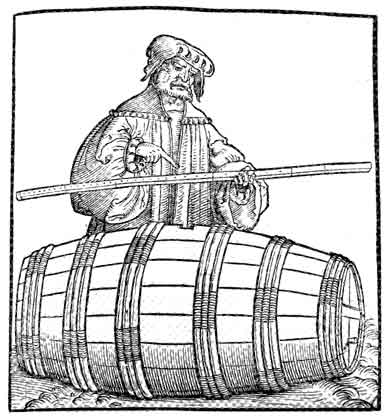
\includegraphics[width=0.382\textwidth]{pictures/fass}
  \end{center}
%\caption{A gull}
\end{wrapfigure}
Die Stereometrie (griech., K\"orpermessung) besch\"aftigt
sich, im Gegensatz zur Planimetrie, mit der Form, gegenseitiger Lage und der Gr\"osse geometrischer Gebilde des Raumes.

Die einfachen K\"orper --- W\"urfel, Quader, Zylinder, Kugel --- waren schon bei allen V\"olkern der vorgeschichtlichen Zeit bekannt und wurden praktisch genutzt. Sowohl die Babyionier (3500 bis 200 v.u.Z.) als auch die \"Agypter (3000 bis 500 v.u.Z.) haben Volumen und Oberfl\"ache von W\"urfeln, Zylindern, Pyramiden und  Kegeln, wenn auch teilweise nur in guter N\"aherung, berechnen k\"onnen. Die Berechnung des Volumens und der Oberfl\"ache einer Kugel gelang aber erst Archimedes (287 - 212 v.u.Z.).

\subsection{Prismen}

\begin{uebenv}{wuerfelundquader}
Berechne Volumen $V$, Oberfl\"ache $O$ und Raumdiagonale $d$ eines
\begin{enumerate}[a)]
\item W\"urfels mit Kantenl\"ange $k$
\item eines Quaders mit Kantenl\"ange $a,b,c$
\end{enumerate}
\end{uebenv}

\subsection{Pyramiden}

\begin{uebenv}{cheops}
Die Cheopspyramide hat als Grundfl\"ache ein Quadrat mit Seitenl\"ange $\unit[233]{m}$. Sie war urspr\"unglich $\unit[148]{m}$ hoch; heute ist sie auf einer H\"ohe von $\unit[137]{m}$ abgestumpft.
\begin{enumerate}[a)]
\item Der Bau soll $\unit[100\,000]{Mann}$ $\unit[20]{Jahre}$ besch\"aftigt haben. Welche Gesteinsmasse wurde dabei bewegt? (Dichte des Gesteins: $\rho_S=\unitfrac[2.7]{g}{cm^3}$)
\item Welche Abmessung hat die heutige Plattform?
\end{enumerate}

\begin{figure}[h!]
\begin{center}
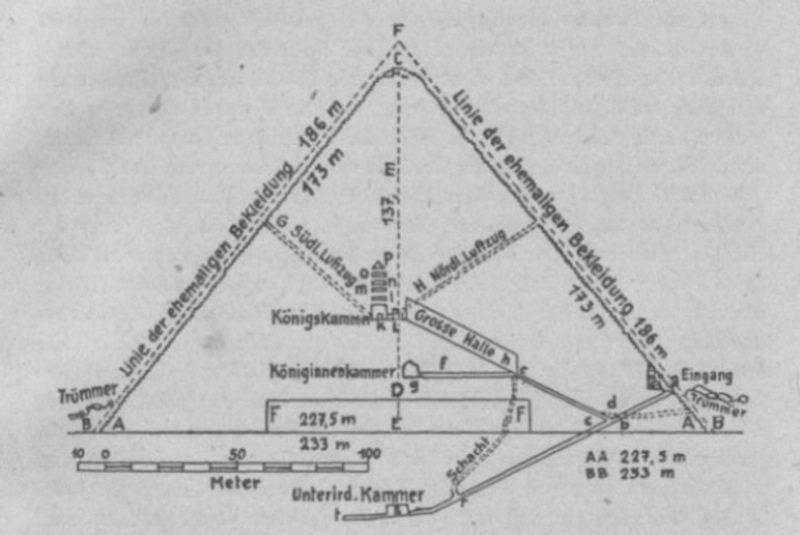
\includegraphics[width=0.9\textwidth]{pictures/cheops}
\caption{Cheopspyramide}
\end{center}
\end{figure}

\end{uebenv}

\subsection{Gerader Kreiszylinder}

\begin{uebenv}{kreiszylinder}
Ein rechteckiges Blatt mit den Seitenl\"angen $a$ und $b$ kann auf zwei Arten zu einem Zylinder gebogen werden. Wie gross ist das Verh\"altnis der (a) Volumina, (b) M\"antel
\end{uebenv}

\begin{uebenv}{konservendose}
Wie viel Blech ben\"otigt man f\"ur eine Konservendose (Durchmesser $\unit[10]{cm}$, Inhalt $\unit[1]{Liter}$), wenn f\"ur Verschnitt etc. noch 15\% zugeschlagen werden?
\end{uebenv}

\begin{uebenv}{kamin}
Die Metallverkleidung eines Kamins muss mit einer Spezialfarbe zweimal gestrichen werden. Die Kaminverkleidung ist ein Zylinder mit einem Durchmesser von $\unit[150]{cm}$ und einer H\"ohe von $\unit[18]{m}$. Beim ersten Anstrich rechnet man mit $\unit[1]{kg}$ Farbe f\"ur $\unit[15]{m^2}$; beim zweiten Anstrich gen\"ugen 70\% der Menge des ersten Anstrichs. Wie viele Dosen ($\unit[5]{kg}$ bzw. $\unit[10]{kg}$) Farbe werden ben\"otigt?
\end{uebenv}

\subsection{Gerader Kreiskegel}

\begin{uebenv}{kreiskegel}
Von einem geraden Kreiskegel kennt man den Radius $r=\unit[5]{cm}$ und das Volumen $V=\unit[1000]{cm^3}$. Berechne $h$, $s$, $M$ und $O$.
\end{uebenv}

\begin{uebenv}{holzkegel}
Wie tief taucht ein Holzkegel ($r=\unit[5]{cm}$, $h=\unit[12]{cm}$, Dichte $\unitfrac[0.8]{g}{cm^3}$) mit der Spitze nach unten in Wasser ein?
\end{uebenv}

\begin{uebenv}{ffnungswinkel}
Wie gross ist der Mittelpunktswinkel des Kreisausschnittes, der den abgewickelten Mantel eines Kegels mit r=6 cm und h=8 cm darstellt?
\end{uebenv}

\begin{uebenv}{kegelvolumen}
Ein Kreisausschnitt mit dem Mittelpunktswinkel 120¡ und dem Radius $\unit[8]{cm}$ wird zu einem Kegel zusammengebogen. Wie gross wird dessen Volumen?
\end{uebenv}

\subsection{Kugel}

Die Berechnung des Volumens der Kugel erfolgt mit dem Prinzip von Cavalieri. Als Vergleichsk\"orper nimmt man denjenigen K\"orper, der entsteht, wenn man aus einem Zylinder (Radius $r$, H\"ohe $r$) einen Kegel herausfr\"ast.
Man schneidet die Halbkugel und den Vergleichsk\"orper mit einer Ebene, die vom Mittelpunkt der Kugel den Abstand $a$ hat. Als Schnittfl\"achen ergeben sich
f\"ur die Halbkugel
$$A = \pi r'^2 =\pi(r^2 - a^2),$$
f\"ur den Vergleichsk\"orper
$$A =A_{Kreisring} =\pi r^2-\pi a^2$$
F\"ur das Volumen der Kugel gilt deshalb:

$$V_{Halbkugel}=V_{Zylinder}-V_{Kegel}
=\pi r^3-\frac{1}{3}\pi r^3=\frac{2}{3}\pi r^3,$$

also
$$V_{Kugel}=\frac{4}{3}\pi r^3.$$

\begin{uebenv}{vkugel}
Berechne den Radius einer Kugel mit $\unit[1]{m^3}$ Rauminhalt.
\end{uebenv}

\begin{uebenv}{hohlkugel}
Leite eine Formel f\"ur das Materialvolumen einer Hohlkugel in Abh\"angigkeit vom Kugelradius $r$ und der Wanddicke $d$ her. Welche Glieder der Formel k\"onnen bei sehr kleinem $d$ vernachl\"assigt werden? Deute die entstehende N\"aherungsformel und leite somit die Formel f\"ur die Oberfl\"ache einer Kugel ab.
\end{uebenv}

\begin{uebenv}{inundumkugel}
Wie verhalten sich die (a) Radien, (b) Oberfl\"achen, (c) Volumina der In- und Umkugel eines W\"urfels?
\end{uebenv}

\clearpage

\subsection{Notizen zu den Übungen}

\begin{lsg}{wuerfelundquader}
\begin{enumerate}[a)]
    \item $V=k^3$, $O=6k^2$, $d=\sqrt{3}k$ (zweimal Pythagoras anwenden)
    \item $V=abc$, $O=2(ab+ac+bc)$, $d=\sqrt{a^2+b^2+c^2}$
\end{enumerate}
\end{lsg}
\begin{lsg}{cheops}
\begin{enumerate}[a)]
    \item Nach dem Strahlensatz gilt für die Plattform $F=\left(\frac{11}{148}\cdot233\right)^2\approx\unit[300]{m^2}$, also hat man eine Seitenlänge von ungefähr 17 Metern.
    \item $V=\frac{1}{3}Gh=\frac{1}{3}\cdot233^2\cdot 148-\frac{1}{3}\cdot(10\sqrt{3})^2\cdot 11\approx2.7\cdot10^6$ mit einer Dichte von $\unitfrac[2.7]{t}{m^3}$. Die Masse ist $m=V\rho\approx7$ Millionen Tonnen.
\end{enumerate}
\end{lsg}
\begin{lsg}{kreiszylinder}
Entweder verwendet man $a$ oder $b$ als Umfang und das zweite für die Höhe. Wegen $U=2\pi r\Leftrightarrow r=\frac{U}{2\pi}$. Die Volumina sind $V_1=(\frac{a}{2\pi})^2b$ und $V_2=(\frac{b}{2\pi})^2a$, woraus $\frac{V_1}{V_2}=\frac{a}{b}$. Die Mäntel ergeben $M_1=M_2$, trivial.
\end{lsg}
\begin{lsg}{konservendose}
Der Radius ist $5$ Centimeter und das Volumen $1000$ Kubikcentimeter, die Höhe daher $h=\frac{1000}{2\pi\cdot5^2}\approx6.4$. Also die Oberfläche ungefähr $357$ Quadratcentimeter; mit $15\%$ Verschnitt sind es $\unit[410]{cm^2}$.
\end{lsg}
\begin{lsg}{kamin}
Der Mantel hat eine Fläche von $\pi\cdot1.5\cdot18\approx\unit[85]{m^2}$ und dazu bräuchte man etwas weniger als $6$ Liter Farbe. Für den zweiten Anstrich $70\%$, was insgesamt etwas weniger als $10$ Liter ergibt
\end{lsg}
\begin{lsg}{kreiskegel}
$V=\frac{1}{3}Gh\Leftrightarrow h=\frac{3V}{G}$ also $h\approx38$ Centimeter. $s=\sqrt{r^2+h^2}\approx39$. Der abgewickelte Mantel ist ein Kreissektor mit Bogenlänge $2\pi r$ und Radius $s$. Sei $\alpha$ der Öffnungswinkel, dann ist $\frac{\alpha}{360^\circ}=\frac{2\pi r}{2\pi s}=\frac{r}{s}$. Für den Mantel gilt also $M=\frac{\alpha}{360^\circ}\cdot\pi s^2=\frac{r}{s}\pi s^2=rs\pi\approx605$ Quadratcentimeter. Die Oberfläche ist $O=684$.
\end{lsg}
\begin{lsg}{holzkegel}
    Der Holzkegel wird schwimmen, da seine Dichte kleiner ist als die Dichte von Wasser. Der Kegel hat die Masse $m_K=80\pi\approx\unit[250]{g}$. Also müssen wir die Höhe des Kegels berechnen, mit der Dichte von Wasser, der $250\,g$ verdrängt. Beachte, dass $\frac{r}{h}=\frac{5}{12}\Leftrightarrow r=\frac{5}{12}h$. Daraus folgt
    $$m_W=\frac{1}{3}\pi\cdot\left(\frac{5}{12}h\right)^2\cdot h\stackrel{!}{=}80\pi\Leftrightarrow h\approx\unit[10.7]{cm}.$$
\end{lsg}
\begin{lsg}{ffnungswinkel}
Die Seitenlänge ist $s=\sqrt{r^2+h^2}=\unit[10]{cm}$. Der abgerollte Kegelmantel, Kreisausschnitt, hat den Radius $s$ und die Bogenlänge $2\pi r$. Den Öffnungswinkel nennen wir $\varphi$. Der Anteil einer vollen Umdrehung ist $\frac{2\pi r}{2\pi s}=\frac{3}{5}$, also ist $\varphi=\frac{3}{5}\cdot360^\circ=216^\circ$.
\end{lsg}
\begin{lsg}{kegelvolumen}
Von vorhin wissen wir, dass $\frac{r}{s}=\frac{\varphi}{360^\circ}$ gilt. Es folgt $s=24$ und $h=\sqrt{s^2-r^2}\approx22.6$. Daraus $V=\frac{1}{3}\pi r^2h\approx1.5$ Liter.
\end{lsg}
\begin{lsg}{vkugel}
Es ist $V_K=\frac{4}{3}\pi r^3\Leftrightarrow r^3=\frac{3V_K}{4\pi}\Leftrightarrow r=\sqrt[3]{\frac{3V_K}{4\pi}}$, also $r\approx 0.24$ Meter.
\end{lsg}
\begin{lsg}{hohlkugel}
Die äussere Hülle hat ein Volumen von $V_a=\frac{4}{3}\pi r^3$ und die innere $V_i=\frac{4}{3}\pi (r-d)^3$. Für das Volumen der Hohlkugel gilt
$$V=V_a-V_i=\frac{4}{3}\pi r^3-\left(\frac{4}{3}\pi r^3-4\pi r^2d+4\pi rd^2-\frac{4}{3}\pi d^3\right)=4\pi d\left(r^2-rd+\frac{\pi}{3}d^2\right).$$
Wird nun $d\to0$ klein, so werden die Terme mit grösseren Exponenten rascher klein als solche mit kleineren Exponenten. Vermutlich dominiert also für kleine $d$ der Term $4\pi dr^2$. Vermutlich ist also $O_K=4\pi r^2$.
\end{lsg}
\begin{lsg}{inundumkugel}
Sei $k$ die Kantenlänge des Würfels. Dann hat die Innkugel Radius $r_i=\frac{k}{2}$ und die Umkugel $r_u=\frac{\sqrt{3}k}{2}=\sqrt{3}r_i$. Also $\frac{r_u}{r_i}=\sqrt{3}$, $\frac{O_a}{O_i}=3$ und $\frac{V_a}{V_i}=3\sqrt{3}$.
\end{lsg}

\clearpage

\section{Ähnlichkeit}

\subsection{Kongruenzabbildungen}
\begin{wrapfigure}{r}{0.382\textwidth}
  \begin{center}
    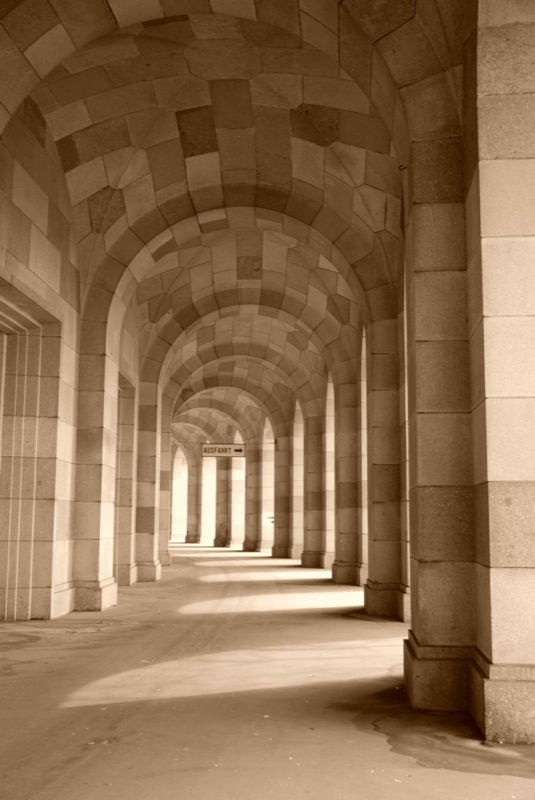
\includegraphics[width=0.382\textwidth]{pictures/torbogen}
  \end{center}
%\caption{A gull}
\end{wrapfigure}
Eine \definition{Abbildung} ist eine eindeutige Zuordnung, bei der jedem Punkt einer ersten Punktmenge genau ein Punkt einer zweiten Punktmenge zugeordnet wird.

Wir nennen die erste Punktmenge die \definition{Urbilder} und die zweite Punktmenge die \definition{Bilder}. In der Regel bezeichnen wir die Bildpunkte zu den Urbildpunkten $A$, $B$, $P$, \dots\ mit $A'$, $B'$, $P'$, \dots.\\

Abbildungen, bei denen die Bilder deckungsgleich (kongruent) zu den Urbildern ist, heissen Kongruenzabbildungen. Kongruente Figuren haben also dieselbe Form und dieselbe Gr\"osse. Zu den Kongruenzabbildungen geh\"oren
\begin{itemize}
\item Achsenspiegelungen
\item Rotationen
\item Punktspiegelungen
\item Translationen
\end{itemize}

\subsection{Zentrische Streckung}
Wir w\"ahlen einen Punkt $Z$ der Ebene und eine positive Zahl $k$. Ordnen wir nun jedem Punkt $P$ einen Bildpunkt $P'$ zu gem\"ass der Vorschrift
\begin{itemize}
\item $P'$ liegt auf dem Strahl $ZP$
\item Die Strecke $ZP'$ ist $k$-mal so lang wie die Strecke $ZP$
\end{itemize}
so heisst diese Abbildung eine \definition{zentrische Streckung} mit dem Streckungszentrum $Z$ und dem Streckungfaktor $k$.%\\[7cm]

Eine zentrische Streckung hat folgende Eigenschaften
\begin{itemize}
\item Urbildwinkel und Bildwinkel sind gleich gross.
\item Urbildgerade und Bildgerade sind parallel.
\item Die Bildstrecke ist $k$-mal so lang wie die Urbildstrecke.
\item Der Fl\"acheninhalt der Bildfigur ist $k^2$-mal so gross wie der Fl\"acheninhalt der Urbildfigur.
\end{itemize}

\begin{uebenv}{zentrischstrecken}
Strecke ein Quadrat $Q$ von einem Punkt $Z$ aus mit dem Streckungsfaktor $3$ zentrisch und \"uberpr\"ufe anschliessend obige Eigenschaften.%\\[8cm]
\end{uebenv}

\begin{uebenv}{negativestreckung}
Eine Streckung mit einem negativen Streckungsfaktor bedeutet eine Streckung mit dem entgegengesetzten positiven Streckungsfaktor und eine zus\"atzliche Punktspiegelung am Streckungszentrum.

\noindent Strecke ein Dreieck von $Z$ aus mit dem Streckungsfaktor $-\frac{1}{2}$.
\end{uebenv}

\subsection{\"Ahnlichkeitsabbildungen}

Kongruenzabbildungen, zentrische Streckungen und ihre Verkettungen heissen \"Ahnlichkeitsabbildungen. Figuren, welche durch \"Ahnlichkeitsabbildungen auseinander hervorgehen, heissen zueinander \definition{\"ahnlich}.

Eine \"Ahnlichkeitsabbildung hat folgende Eigenschaften
\begin{itemize}
\item Urbildwinkel und Bildwinkel sind gleich gross.
\item Alle Bildstrecken sind $k$-mal so lang wie die entsprechenden Urbildstrecken.
\item Der Fl\"acheninhalt der Bildfigur ist $k^2$-mal so gross wie der Fl\"acheninhalt der Urbildfigur
\end{itemize}

\begin{bem}
    Daraus folgt insbesondere f\"ur \"ahnliche Dreiecke, dass sie gleiche Winkel haben und im Verh\"altnis von zwei einander entsprechenden Seiten \"ubereinstimmen.
\end{bem}

\begin{uebenv}{kreisesindhnlich}
Alle Kreise sind zueinander \"ahnlich. Wie verhalten sich die Fl\"achen zweier Kreise, wenn sich ihre Radien wie $2\div3$ verhalten?
\end{uebenv}

\subsection{Strahlens\"atze}

\begin{csatz}[1. Strahlensatz]
Werden zwei Strahlen mit gemeinsamem Anfangspunkt von zwei Parallelen geschnitten, so verhalten sich die Abschnitte auf dem einen Strahl wie die entsprechenden Abschnitte auf dem andern Strahl.%\\[6cm]
\end{csatz}

\begin{center}
    \begin{tikzpicture}[scale=1.2]

    % Farben für bessere Visualisierung
    \definecolor{raycolor}{rgb}{0.2, 0.6, 0.8}
    \definecolor{parallelcolor}{rgb}{0.8, 0.3, 0.3}
    \definecolor{pointcolor}{rgb}{0.1, 0.5, 0.2}

    % Grundpunkte
    \coordinate (A) at (0, 0); % Scheitelpunkt
    \coordinate (B) at (3, 2); % Punkt auf erstem Strahl (unten)
    \coordinate (C) at (5, 3.333); % Punkt auf erstem Strahl (oben)
    \coordinate (D) at (3, -1.5); % Punkt auf zweitem Strahl (unten)
    \coordinate (E) at (5, -2.5); % Punkt auf zweitem Strahl (oben)

    % Parallelen zeichnen
    \draw[parallelcolor, thick] (3, 2.5) -- (3,-2) node[pos=0.5, right] {$g$};
    \draw[parallelcolor, thick] (5, 3.5) -- (5, -3) node[pos=0.5, right] {$h$};

    % Strahlen
    \draw[raycolor, thick] (A) -- (C);
    \draw[raycolor, thick] (A) -- (E);

    % Punkte einfügen
    \fill[pointcolor] (A) circle (2pt) node[below left] {$A$};
    \fill[pointcolor] (B) circle (2pt) node[above left] {$B$};
    \fill[pointcolor] (C) circle (2pt) node[above left] {$C$};
    \fill[pointcolor] (D) circle (2pt) node[below left] {$D$};
    \fill[pointcolor] (E) circle (2pt) node[below left] {$E$};

    % Markierungen einfügen
    \draw[<->, thick] (A) -- (B) node[midway, above left] {$a$};
    \draw[<->, thick] (B) -- (C) node[midway, above left] {$b$};
    \draw[<->, thick] (A) -- (D) node[midway, below left] {$c$};
    \draw[<->, thick] (D) -- (E) node[midway, below left] {$d$};

\end{tikzpicture}
\end{center}

\begin{uebenv}{strecketeilen}
Teile eine Strecke im Verh\"altnis $2\div3$.
\end{uebenv}

\begin{csatz}[2. Strahlensatz]
Werden zwei Strahlen mit gemeinsamem Anfangspunkt von zwei Parallelen geschnitten, so verhalten sich die Parallelenabschnitte wie die vom Anfangspunkt aus gemessenen Abschnitte auf einem der Strahlen.%\\[6cm]
\end{csatz}

\begin{uebenv}{beweisstrahlensatz}
    Beweise folgende Aussagen:
    \begin{enumerate}[a)]
        \item $\frac{a}{a+b}=\frac{c}{c+d}$
        \item $\frac{a}{g}=\frac{a+b}{h}$
        \item $\frac{a}{b}=\frac{c}{d}$
    \end{enumerate}
\end{uebenv}

\begin{uebenv}{telefonstange}
Eine freistehende Telefonstange im ebenen Gel\"ande wirft bei einem bestimmten Sonnenstand einen Schatten von $\unit[5.6]{m}$ L\"ange. Um die Stangenh\"ohe $h$ zu bestimmen, wird ein Meterstab parallel zur Stange aufgestellt, so dass beide Schattengrenzen zusammenfallen. Der Abstand des Meterstabes von der Stange misst $\unit[2.9]{m}$.
\end{uebenv}

\subsection{\"Ahnliche K\"orper}

K\"orper, welche durch \"Ahnlichkeitsabbildungen auseinander hervorgehen, heissen zueinander \"ahnlich.

Neben den bereits bekannten Eigenschaften von \"Ahnlichkeitsabbildungen gilt zusätzlich: Das Volumen des Bildk\"orpers ist $k^3$-mal so gross wie das Volumen des Urbildk\"orpers%\\[6cm]

\begin{bsp}
Alle W\"urfel sind zueinander \"ahnlich.
\end{bsp}

\begin{bsp}

\begin{enumerate}[a)]
\item Zwei W\"urfel aus gleichem Material wiegen $\unit[1]{g}$ und $\unit[1]{kg}$. Der leichtere W\"urfel hat eine Kantenl\"ange von $\unit[5]{cm}$. Wie lang ist eine Kante des schwereren W\"urfels?

Weil die beiden W\"urfel aus gleichem Material sind verhalten sich wegen
$$\frac{m_1}{m_2}=\frac{V_1\cdot\rho}{V_2\cdot\rho}=\frac{V_1}{V_2}$$
ihre Volumina wie $1\div1000$, also wegen $10^3=1000$ ihre Kantenl\"angen wie $1\div10$. Die Kantenl\"ange des schwereren W\"urfels betr\"agt deshalb $\unit[50]{cm}$.

\item Ein gerader Kreiskegel wird durch einen Schnitt parallel zur Grundfl\"ache in halber H\"ohe geteilt. Er zerf\"allt dabei in einen kleineren Kegel und einen Kegelstumpf. Wie verhalten sich die Volumina der beiden Teile?

Der kleine Kegel ist zum urspr\"unglichen \"ahnlich (zentrische Streckung mit Kegelspitze als Streckungszentrum). Ihre H\"ohen verhalten sich wie $1\div2$, ihre Grundfl\"achen wie $1\div4$ und ihre Volumina wie $1\div8$. Das Volumen des Kegelstumpfs ist Volumen des urspr\"unglichen Kegels minus Volumen des kleinen Kegels. Also verh\"alt sich das Volumen des kleinen Kegels zu dem des Kegelstumpfs wie $1\div7$.
\end{enumerate}
\end{bsp}

\clearpage

\subsection{Notizen zu den Übungen}

\begin{lsg}{zentrischstrecken}
\begin{center}
    \begin{tikzpicture}
    % Originales Quadrat Q
    \draw[thick] (0,0) rectangle (2,2);
    \node at (1,1) {$Q$};

    % Punkt Z
    \fill (0,0) circle (2pt);
    \node[below left] at (0,0) {$Z$};

    % Gestrecktes Quadrat
    \begin{scope}[shift={(3,3)}, scale=3]
        \draw[dashed, thick] (-1,-1) rectangle (1,1);
        \node at (0,0) {$Q'$};
    \end{scope}
\end{tikzpicture}
\end{center}
\end{lsg}
\begin{lsg}{negativestreckung}
\begin{center}
    \begin{tikzpicture}
    % Originales Dreieck
    \draw[thick] (0,0) -- (2,0) -- (1,2) -- cycle;
    \node at (1,0.5) {$D$};

    % Punkt Z
    \fill (2,2) circle (2pt);
    \node[above left] at (2,2) {Z};

    % Gestrecktes Dreieck
    \begin{scope}[shift={(3,3)}, scale=-0.5]
        \draw[dashed, thick] (0,0) -- (2,0) -- (1,2) -- cycle;
        \node at (1,0.5) {$D'$};
    \end{scope}
\end{tikzpicture}
\end{center}
\end{lsg}
\begin{lsg}{kreisesindhnlich}
Kreise gehen durch zentrische Streckung am Mittelpunkt ineinander über. Gegebenenfalls müssen die Mittelpunkte zuerst mit einer Translation zur Deckung gebracht werden.

Flächen sind zweidimensional, also verhalten sie sich wie $\left(\frac{2}{3}\right)^2=4\div9$.
\end{lsg}
\begin{lsg}{strecketeilen}
Gegeben sei eine Strecke mit Anfangspunkt $A$ und Endpunkt $B$. Zeichne einen Strahl von $A$ aus und unterteile ihn in fünf beliebig, aber gleich grosse Abschnitte. Verbinde die letzte Markierung mit dem Punkt $B$. Verschiebe diese Strecke parallel, bis sie die vorletzte Markierung auf dem Strahl schneidet. Der Schnittpunkt dieser Parallelen mit der Strecke $AB$ teilt diese im Verhältnis $2\div3$
\end{lsg}
\begin{lsg}{beweisstrahlensatz}
Man kann die Strahlen auch mit Geraden formulieren und dann mit Schnittpunkten arbeiten. Daraus ergeben sich dann mit Hilfe der Koordinaten dieser Schnittpunkte und dem Satz von Pythagoras die obigen Gleichheiten.

Wir betrachten ein Ähnlichkeitsargument:
    \begin{enumerate}[a)]
        \item Sei $a+b=k\cdot a$ eine zentrische Streckung. Dann gilt auch $c+d=kc$, da die Dreiecke $ABD$ und $AEC$ ähnlich sind. Es folgt
        $$\frac{a}{a+b}=\frac{a}{ka}=\frac{1}{k}=\frac{c}{kc}=\frac{c}{c+d}$$

        \item Diese Beziehung ergibt sich analog zur ersten auf Grund der Ähnlichkeit der Dreiecke.

        \item Hier können wir nicht mit einer zentrischen Streckung arbeiten. Aber aus der ersten Gleichheit folgt
        $$a(c+d)=c(a+b)\Leftrightarrow ac+ad=ca+cb\Leftrightarrow ad=cb\Leftrightarrow \frac{a}{b}=\frac{c}{d}.$$
    \end{enumerate}
\end{lsg}
\begin{lsg}{telefonstange}
Wir haben die Gleichung $\frac{1}{2.7}=\frac{h}{5.6}$, woraus unmittelbar $h=\frac{5.6}{2.7}\approx2.1\,\text{m}$ folgt.
\end{lsg}

\subsection{Übungen}

\begin{enumerate}
\item Spiegle das Dreieck und den Kreis an der Geraden $g$.\\
\begin{center}
\scalebox{1.3}{
\begin{tikzpicture}[line cap=round,line join=round,>=triangle 45,x=0.7cm,y=0.7cm]
\clip(-4.22,-3.2) rectangle (6.84,5.64);
\draw [line width=1.6pt,domain=-4.22:6.84] plot(\x,{(--18.3-3.62*\x)/10.7});
\draw [line width=2pt] (0.96,1.39)-- (-0.58,5.4);
\draw [line width=2pt] (-0.58,5.4)-- (-0.72,1.1);
\draw [line width=2pt] (-0.72,1.1)-- (0.96,1.39);
\draw [line width=1.6pt] (3.6,-1.7) circle (0.8cm);
\draw[color=black] (-3.24,2.36) node {$g$};
\fill [color=black] (3.6,-1.7) circle (1.5pt);
\end{tikzpicture}
}
\end{center}
\item Die Figur $F$ kann durch eine Achsenspiegelung in die Figur $F'$ \"uberf\"uhrt werden. Konstruiere die Spiegelachse.\\
\begin{center}
\scalebox{1.2}{
\begin{tikzpicture}[line cap=round,line join=round,>=triangle 45,x=1cm,y=1cm]
\clip(-3.17,-2.47) rectangle (4.08,2.91);
\draw [line width=1.6pt] (-1.98,-1.86)-- (-2.22,-0.14);
\draw [line width=1.6pt] (-2.22,-0.14)-- (0.64,-2.18);
\draw [line width=1.6pt] (3.33,1.56)-- (1.86,2.49);
\draw [line width=1.6pt] (1.86,2.49)-- (2.54,-0.96);
\draw (-2.79,-0.69) node[anchor=north west] {$F'$};
\draw (3.1,2.3) node[anchor=north west] {$F$};
\end{tikzpicture}
}
\end{center}

\item Geht eine Figur durch eine Achsenspiegelung in sich selbst \"uber, so heisst die Figur achsensymmetrisch. Bei Achsensymmetrie heisst die Spiegelachse auch Symmetrieachse der Figur.

Zeichne bei den Figuren alle m\"oglichen Symmetrieachsen und Symmetriepunkte ein.\\
\begin{center}
\scalebox{1.1}{
\begin{tikzpicture}[line cap=round,line join=round,>=triangle 45,x=0.9cm,y=0.75cm]
\clip(-4.7,-0.9) rectangle (8,2.84);
\draw [line width=2pt] (-4,2)-- (-1,2);
\draw [line width=2pt] (-1,2)-- (-1,0);
\draw [line width=2pt] (-1,0)-- (-4,0);
\draw [line width=2pt] (-4,0)-- (-4,2);
\draw [line width=2pt] (1,-0.5)-- (1,1.5);
\draw [line width=2pt] (1,1.5)-- (4,2.5);
\draw [line width=2pt] (4,2.5)-- (4,0.5);
\draw [line width=2pt] (4,0.5)-- (1,-0.5);
\draw [line width=2pt] (5,2)-- (7,2);
\draw [line width=2pt] (7,2)-- (7,0);
\draw [line width=2pt] (7,0)-- (5,0);
\draw [line width=2pt] (5,0)-- (5,2);
\end{tikzpicture}
}
\end{center}

\item Drehe den Punkt $P$ um $Z$ um den Winkel $120^\circ$ im Uhrzeigersinn.\\
\begin{center}
\scalebox{1.1}{
\begin{tikzpicture}[line cap=round,line join=round,>=triangle 45,x=1.368cm,y=1.368cm]
\clip(-2.66,-0.56) rectangle (3.92,1.08);
\fill [color=black] (-1.39,0.3) circle (1.5pt);
\draw[color=black] (-1.27,0.52) node {$P$};
\fill [color=black] (1.67,0.25) circle (1.5pt);
\draw[color=black] (1.78,0.47) node {$Z$};
\end{tikzpicture}
}
\end{center}

\item Der Punkt $A$ wurde um einen Drehpunkt nach $A'$ gedreht. Wo muss der Drehpunkt liegen?
\begin{center}
\scalebox{1}{
\begin{tikzpicture}[line cap=round,line join=round,>=triangle 45,x=0.7974481658692185cm,y=0.7943925233644861cm]
\clip(-4.3,2.02) rectangle (8.24,6.3);
\fill [color=black] (-2,3) circle (1.5pt);
\draw[color=black] (-1.84,3.4) node {$A$};
\fill [color=black] (4.56,3.84) circle (1.5pt);
\draw[color=black] (4.74,4.26) node {$A'$};
\end{tikzpicture}
}
\end{center}

\item Die Strecke $AB$ wurde um einen Drehpunkt nach $A'B'$ gedreht. Konstruiere den Drehpunkt.\\
\begin{center}
\scalebox{0.8}{
\begin{tikzpicture}[line cap=round,line join=round,>=triangle 45,x=0.75cm,y=0.75cm]
\clip(-4.3,-1.54) rectangle (7.86,6.3);
\draw [line width=2pt] (-2.16,0.22)-- (-0.42,3.98);
\draw [line width=2pt] (6.1,0.82)-- (3.58,4.1);
\draw (-2.8,0.8) node[anchor=north west] {$A$};
\draw (-0.9,4.68) node[anchor=north west] {$B$};
\draw (3.68,4.8) node[anchor=north west] {$A'$};
\draw (6.26,1.24) node[anchor=north west] {$B'$};
\end{tikzpicture}
}
\end{center}

\item Eine rechteckige Tischplatte soll auf ihrem Untergestell derart gelagert sein, dass sie die beiden gezeichneten Lagen einnehmen kann. An welcher Stelle muss der Tischler den Drehzapfen anbringen?\\
\begin{center}
\begin{tikzpicture}[line cap=round,line join=round,>=triangle 45,x=0.75cm,y=0.75cm]
\clip(-3.96,-0.84) rectangle (5.4,6.72);
\draw [line width=2pt] (-3,0)-- (3,0);
\draw [line width=2pt] (3,0)-- (3,2);
\draw [line width=2pt] (3,2)-- (-3,2);
\draw [line width=2pt] (-3,2)-- (-3,0);
\draw [line width=2pt,dash pattern=on 4pt off 4pt] (-1,6)-- (1,6);
\draw [line width=2pt,dash pattern=on 4pt off 4pt] (1,6)-- (1,0);
\draw [line width=2pt,dash pattern=on 4pt off 4pt] (1,0)-- (-1,0);
\draw [line width=2pt,dash pattern=on 4pt off 4pt] (-1,0)-- (-1,6);
\end{tikzpicture}
\end{center}


\item Ein Sportflugzeug fliegt mit einer Geschwindigkeit von $\unitfrac[240]{km}{h}$ nach Norden. Von Westen weht ein Wind mit $\unitfrac[60]{km}{h}$. Bestimmen an der Abbildung die Richtung und die tats\"achliche Geschwindigkeit des Flugzeugs gegen\"uber dem Erdboden.\\
\begin{center}
\scalebox{0.95}{
\begin{tikzpicture}[line cap=round,line join=round,>=triangle 45,x=1.04cm,y=1.04cm]
\clip(-1.12,-0.16) rectangle (1.76,4.3);
\draw [->,line width=1.6pt] (0,0) -- (1,0);
\draw [->,line width=1.6pt] (0,0) -- (0,4);
\draw (0.1,4) node[anchor=north west] {$\unitfrac[240]{km}{h}$};
\draw (0.4,0.7) node[anchor=north west] {$\unitfrac[60]{km}{h}$};
\end{tikzpicture}
}
\end{center}

\item Durch zentrische Streckung mit dem Streckungszentrum $Z$ ist aus dem Originaldreieck $ABC$ das Bilddreieck $A'B'C'$ entstanden.

Mit welchem Streckungsfaktor wurde es gestreckt? In welchem Verh\"altnis stehen entsprechende Seitenl\"angen zueinander? In welchem Verh\"altnis stehen die Fl\"acheninhalte zueinander?\\[-6ex]
\begin{center}
\definecolor{zzttqq}{rgb}{0.6,0.2,0}
\definecolor{wwttqq}{rgb}{0.4,0.2,0}
\definecolor{qqwwcc}{rgb}{0,0.4,0.8}
\definecolor{qqqqzz}{rgb}{0,0,0.6}
\begin{tikzpicture}[line cap=round,line join=round,>=triangle 45,x=0.865cm,y=0.865cm]
\clip(-1.62,-4.9) rectangle (9.94,1.82);
\fill[color=qqwwcc,fill=qqwwcc,fill opacity=0.1] (1.14,-1.62) -- (2.58,-1.92) -- (2.04,-2.58) -- cycle;
\fill[color=zzttqq,fill=zzttqq,fill opacity=0.1] (4.86,-0.66) -- (9.18,-1.56) -- (7.56,-3.54) -- cycle;
\draw [line width=2.4pt,color=qqwwcc] (1.14,-1.62)-- (2.58,-1.92);
\draw [line width=2.8pt,color=qqwwcc] (2.58,-1.92)-- (2.04,-2.58);
\draw [line width=2.4pt,color=qqwwcc] (2.04,-2.58)-- (1.14,-1.62);
\draw [domain=-0.72:9.94] plot(\x,{(-3.56--0.48*\x)/1.86});
\draw [domain=-0.72:9.94] plot(\x,{(-6.8--0.18*\x)/3.3});
\draw [domain=-0.72:9.94] plot(\x,{(-6.14-0.48*\x)/2.76});
\draw [line width=2.4pt,color=zzttqq] (4.86,-0.66)-- (9.18,-1.56);
\draw [line width=2.4pt,color=zzttqq] (9.18,-1.56)-- (7.56,-3.54);
\draw [line width=2.4pt,color=zzttqq] (7.56,-3.54)-- (4.86,-0.66);
\fill [color=black] (-0.72,-2.1) circle (1.5pt);
\draw[color=black] (-0.92,-1.7) node {$Z$};
\fill [color=qqqqzz] (1.14,-1.62) circle (1.5pt);
\draw[color=qqqqzz] (1.18,-1.26) node {$C$};
\fill [color=qqqqzz] (2.58,-1.92) circle (1.5pt);
\draw[color=qqqqzz] (2.72,-1.66) node {$B$};
\fill [color=qqqqzz] (2.04,-2.58) circle (1.5pt);
\draw[color=qqqqzz] (1.88,-2.86) node {$A$};
\fill [color=wwttqq] (4.86,-0.66) circle (1.5pt);
\draw[color=wwttqq] (5,-0.3) node {$C'$};
\fill [color=wwttqq] (9.18,-1.56) circle (1.5pt);
\draw[color=wwttqq] (9.36,-1.3) node {$B'$};
\fill [color=wwttqq] (7.56,-3.54) circle (1.5pt);
\draw[color=wwttqq] (7.44,-3.86) node {$A'$};
\end{tikzpicture}
\end{center}
\item Strecke die Figur von $Z$ aus mit dem Streckungsfaktor $\frac{1}{3}$.\\
\begin{center}
\definecolor{zzttqq}{rgb}{0.6,0.2,0}
\scalebox{1.1}{
\begin{tikzpicture}[line cap=round,line join=round,>=triangle 45,x=0.865cm,y=0.865cm]
\clip(-1.62,-4.9) rectangle (9.94,1.82);
\fill[color=zzttqq,fill=zzttqq,fill opacity=0.1] (-1.02,-2.56) -- (-0.98,-4.7) -- (5.1,-4.74) -- (5.1,-4.02) -- (-0.16,-4.02) -- (-0.2,-2.56) -- cycle;
\draw [color=zzttqq] (-1.02,-2.56)-- (-0.98,-4.7);
\draw [color=zzttqq] (-0.98,-4.7)-- (5.1,-4.74);
\draw [color=zzttqq] (5.1,-4.74)-- (5.1,-4.02);
\draw [color=zzttqq] (5.1,-4.02)-- (-0.16,-4.02);
\draw [color=zzttqq] (-0.16,-4.02)-- (-0.2,-2.56);
\draw [color=zzttqq] (-0.2,-2.56)-- (-1.02,-2.56);
\fill [color=black] (8.92,0.9) circle (1.5pt);
\draw[color=black] (8.7,1.26) node {$Z$};
\end{tikzpicture}
}
\end{center}

\item Strecke das Rechteck von $Z$ aus mit dem Streckungsfaktor $-2$.\\
\begin{center}
\definecolor{zzttqq}{rgb}{0.6,0.2,0}
\definecolor{zzzzzz}{rgb}{0.6,0.6,0.6}
\scalebox{0.9}{
\begin{tikzpicture}[line cap=round,line join=round,>=triangle 45,x=0.93cm,y=0.93cm]
\draw [color=zzzzzz,dash pattern=on 2pt off 2pt, xstep=0.93cm,ystep=0.93cm] (0.56,-6.52) grid (15.62,1.4);
\clip(0.56,-6.52) rectangle (15.62,1.4);
\fill[color=zzttqq,fill=zzttqq,fill opacity=0.1] (3,0) -- (7,0) -- (7,-2) -- (3,-2) -- cycle;
\draw [color=zzttqq] (3,0)-- (7,0);
\draw [color=zzttqq] (7,0)-- (7,-2);
\draw [color=zzttqq] (7,-2)-- (3,-2);
\draw [color=zzttqq] (3,-2)-- (3,0);
\fill [color=black] (7,-2) circle (1.5pt);
\draw[color=black] (6.8,-2.32) node {$Z$};
\end{tikzpicture}
}
\end{center}

\item Verbindet man die Seitenmitten eines Dreiecks $ABC$, so entsteht ein weiteres Dreieck. Dieses k\"onnte aus dem Dreieck $ABC$ durch eine zentrische Streckung erhalten werden. Wo liegt das Streckungszentrum und wie gross ist der Streckungsfaktor?

\item In einem Zimmer steht das schwarze rechteckige Brett parallel zur Wand auf dem Boden. Von einem Punkt vom Boden aus strahlt Licht. Zeichnen Sie die Lichtstrahlen durch die oberen Eckpunkte des Bretts und finde so deren Schlagschatten an der Wand.\\
\begin{center}
\definecolor{zzttqq}{rgb}{0.6,0.2,0}
\definecolor{ccccqq}{rgb}{0.8,0.8,0}
\scalebox{0.9}{
\begin{tikzpicture}[line cap=round,line join=round,>=triangle 45,x=0.9124cm,y=0.9124cm]
\clip(2.22,-7.84) rectangle (13.18,-0.04);
\fill[fill=black,fill opacity=1.0] (6.9,-4.34) -- (7.58,-5.47) -- (7.6,-4.28) -- (6.86,-3.22) -- cycle;
\fill[color=zzttqq,fill=zzttqq,fill opacity=0.1] (9.5,-3.44) -- (11.2,-5.8) -- (7.58,-5.47) -- (7.6,-4.28) -- (7.5,-4.13) -- cycle;
\draw (2.54,-6.8)-- (11.92,-6.8);
\draw (11.92,-6.8)-- (11.84,-0.5);
\draw (11.92,-6.8)-- (8.54,-2.12);
\draw (8.54,-2.12)-- (8.56,-0.58);
\draw (8.54,-2.12)-- (4.14,-2.1);
\draw (4.46,-5.18)-- (11.2,-5.8);
\draw (4.46,-5.18)-- (9.5,-3.44);
\draw (6.9,-4.34)-- (7.58,-5.47);
\draw (7.58,-5.47)-- (7.6,-4.28);
\draw (7.6,-4.28)-- (6.86,-3.22);
\draw (6.86,-3.22)-- (6.9,-4.34);
\draw [color=zzttqq] (9.5,-3.44)-- (11.2,-5.8);
\draw [color=zzttqq] (11.2,-5.8)-- (7.58,-5.47);
\draw [color=zzttqq] (7.58,-5.47)-- (7.6,-4.28);
\draw [color=zzttqq] (7.6,-4.28)-- (7.5,-4.13);
\draw [color=zzttqq] (7.5,-4.13)-- (9.5,-3.44);
\fill [color=ccccqq] (4.46,-5.18) circle (1.5pt);
\end{tikzpicture}
}
\end{center}
\item Ein Filmnegativ der Gr\"osse $\unit[24\times36]{mm}$ soll so vergr\"ossert werden, dass das Bild alles zeigt, was auf dem Negativ ist. Bei welchem der drei Papierformate $9\times13$, $10\times15$, $13\times18$ (alle Masse in $\unit{cm}$) ist dies ohne Verschnitt m\"oglich?

\item Der Kreis mit Mittelpunkt $M$ soll von $Z$ aus so gestreckt werden, dass der Bildkreis die Gerade $g$ ber\"uhrt. Konstruiere den Bildkreis.
\begin{center}
<<<<<<< Updated upstream
\definecolor{qqqqff}{rgb}{0,0,1}
=======

>>>>>>> Stashed changes
\scalebox{0.9}{
\begin{tikzpicture}[line cap=round,line join=round,>=triangle 45,x=0.7353cm,y=0.7353cm]
\clip(0.52,-6.76) rectangle (16.84,0.36);
\draw [line width=1.6pt] (7.54,-0.4)-- (16.12,-3.18);
\draw [line width=1.6pt] (6.42,-3.68) circle (1.47cm);
\fill [color=black] (6.42,-3.68) circle (1.5pt);
\draw[color=black] (6.16,-3.96) node {$M$};
<<<<<<< Updated upstream
\fill [color=qqqqff] (0.94,-1.8) circle (1.5pt);
\draw[color=qqqqff] (0.72,-1.4) node {$Z$};
=======
\fill [color=darkblue] (0.94,-1.8) circle (1.5pt);
\draw[color=darkblue] (0.72,-1.4) node {$Z$};
>>>>>>> Stashed changes
\end{tikzpicture}
}
\end{center}

\item Auf einer Karte mit Massstab $1\div25'000$ ist ein horizontales Autobahnst\"uck $\unit[65]{mm}$ lang und eine Stadt bedeckt eine Fl\"ache von $\unit[420]{cm^2}$. Wie lang ist das Autobahnst\"uck und wie gross ist die Stadtfl\"ache in Wirklichkeit?
\item Die Schweiz hat eine Fl\"ache von $\unit[41'000]{km^2}$. Die Luftlinie Bern-Thun betr\"agt $\unit[25]{km}$. Welche Fl\"ache hat die Schweiz auf einer Karte, bei der die Distanz Bern-Thun $\unit[5]{cm}$ betr\"agt?

\item Die Originalfigur $A$ kann je durch eine \"Ahnlichkeitsabbildung in die Bildfigur $B$, $C$, $D$, $E$, $F$ oder $G$ abgebildet werden.
\begin{center}
\definecolor{zzttqq}{rgb}{0.6,0.2,0}
\definecolor{wwwwww}{rgb}{0.4,0.4,0.4}
\scalebox{0.7}{
\begin{tikzpicture}[line cap=round,line join=round,>=triangle 45,x=1cm,y=1cm]
\draw [color=wwwwww,dash pattern=on 2pt off 2pt, xstep=0.5cm,ystep=0.5cm] (-4.3,-5.24) grid (10.2,6.3);
\clip(-4.3,-5.24) rectangle (10.42,6.3);
\fill[color=zzttqq,fill=zzttqq,fill opacity=0.1] (-3.5,5.5) -- (-0.5,5.5) -- (-0.5,3.5) -- (-1.5,3.5) -- (-1.5,4.5) -- (-3.5,4.5) -- cycle;
\fill[color=zzttqq,fill=zzttqq,fill opacity=0.1] (3.5,3.5) -- (3.5,5.5) -- (6.5,5.5) -- (6.5,4.5) -- (4.5,4.5) -- (4.5,3.5) -- cycle;
\fill[color=zzttqq,fill=zzttqq,fill opacity=0.1] (0.5,2.5) -- (2.5,2.5) -- (2.5,-0.5) -- (1.5,-0.5) -- (1.5,1.5) -- (0.5,1.5) -- cycle;
\fill[color=zzttqq,fill=zzttqq,fill opacity=0.1] (-3,0.5) -- (-1.5,0.5) -- (-1.5,0) -- (-2.5,0) -- (-2.5,-0.5) -- (-3,-0.5) -- cycle;
\fill[color=zzttqq,fill=zzttqq,fill opacity=0.1] (-1.5,-1.5) -- (-0.5,-1.5) -- (-0.5,-3.5) -- (-3.5,-3.5) -- (-3.5,-2.5) -- (-1.5,-2.5) -- cycle;
\fill[color=zzttqq,fill=zzttqq,fill opacity=0.1] (6.5,2.5) -- (9.5,2.5) -- (9.5,1.5) -- (7.5,1.5) -- (7.5,0.5) -- (6.5,0.5) -- cycle;
\fill[color=zzttqq,fill=zzttqq,fill opacity=0.1] (7,-1.5) -- (8.5,-1.5) -- (8.5,-4.5) -- (4,-4.5) -- (4,-3) -- (7,-3) -- cycle;
\draw [color=zzttqq] (-3.5,5.5)-- (-0.5,5.5);
\draw [color=zzttqq] (-0.5,5.5)-- (-0.5,3.5);
\draw [color=zzttqq] (-0.5,3.5)-- (-1.5,3.5);
\draw [color=zzttqq] (-1.5,3.5)-- (-1.5,4.5);
\draw [color=zzttqq] (-1.5,4.5)-- (-3.5,4.5);
\draw [color=zzttqq] (-3.5,4.5)-- (-3.5,5.5);
\draw [color=zzttqq] (3.5,3.5)-- (3.5,5.5);
\draw [color=zzttqq] (3.5,5.5)-- (6.5,5.5);
\draw [color=zzttqq] (6.5,5.5)-- (6.5,4.5);
\draw [color=zzttqq] (6.5,4.5)-- (4.5,4.5);
\draw [color=zzttqq] (4.5,4.5)-- (4.5,3.5);
\draw [color=zzttqq] (4.5,3.5)-- (3.5,3.5);
\draw [color=zzttqq] (0.5,2.5)-- (2.5,2.5);
\draw [color=zzttqq] (2.5,2.5)-- (2.5,-0.5);
\draw [color=zzttqq] (2.5,-0.5)-- (1.5,-0.5);
\draw [color=zzttqq] (1.5,-0.5)-- (1.5,1.5);
\draw [color=zzttqq] (1.5,1.5)-- (0.5,1.5);
\draw [color=zzttqq] (0.5,1.5)-- (0.5,2.5);
\draw [color=zzttqq] (-3,0.5)-- (-1.5,0.5);
\draw [color=zzttqq] (-1.5,0.5)-- (-1.5,0);
\draw [color=zzttqq] (-1.5,0)-- (-2.5,0);
\draw [color=zzttqq] (-2.5,0)-- (-2.5,-0.5);
\draw [color=zzttqq] (-2.5,-0.5)-- (-3,-0.5);
\draw [color=zzttqq] (-3,-0.5)-- (-3,0.5);
\draw [color=zzttqq] (-1.5,-1.5)-- (-0.5,-1.5);
\draw [color=zzttqq] (-0.5,-1.5)-- (-0.5,-3.5);
\draw [color=zzttqq] (-0.5,-3.5)-- (-3.5,-3.5);
\draw [color=zzttqq] (-3.5,-3.5)-- (-3.5,-2.5);
\draw [color=zzttqq] (-3.5,-2.5)-- (-1.5,-2.5);
\draw [color=zzttqq] (-1.5,-2.5)-- (-1.5,-1.5);
\draw [color=zzttqq] (6.5,2.5)-- (9.5,2.5);
\draw [color=zzttqq] (9.5,2.5)-- (9.5,1.5);
\draw [color=zzttqq] (9.5,1.5)-- (7.5,1.5);
\draw [color=zzttqq] (7.5,1.5)-- (7.5,0.5);
\draw [color=zzttqq] (7.5,0.5)-- (6.5,0.5);
\draw [color=zzttqq] (6.5,0.5)-- (6.5,2.5);
\draw [color=zzttqq] (7,-1.5)-- (8.5,-1.5);
\draw [color=zzttqq] (8.5,-1.5)-- (8.5,-4.5);
\draw [color=zzttqq] (8.5,-4.5)-- (4,-4.5);
\draw [color=zzttqq] (4,-4.5)-- (4,-3);
\draw [color=zzttqq] (4,-3)-- (7,-3);
\draw [color=zzttqq] (7,-3)-- (7,-1.5);
\draw (-0.36,5.18) node[anchor=north west] {B};
\draw (3,5.28) node[anchor=north west] {A};
\draw (0.62,3) node[anchor=north west] {C};
\draw (-3.5,0.38) node[anchor=north west] {E};
\draw (6,2.26) node[anchor=north west] {D};
\draw (-0.32,-1.74) node[anchor=north west] {F};
\draw (8.72,-2.08) node[anchor=north west] {G};
\end{tikzpicture}
}
\end{center}
Welche Abbildung ist
\begin{enumerate}[a)]
\item eine Kongruenzabbildung
\item eine Punktspiegelung
\item eine Rotation
\item eine Achsenspiegelung
\item eine Verschiebung
\item eine zentrische Streckung
\end{enumerate}
\item Welche Figuren sind zueinander \"ahnlich?
\begin{center}
\definecolor{zzttqq}{rgb}{0.6,0.2,0}
\definecolor{zzzzzz}{rgb}{0.6,0.6,0.6}
\scalebox{0.9}{
\begin{tikzpicture}[line cap=round,line join=round,>=triangle 45,x=0.733cm,y=0.733cm]
\draw [color=zzzzzz,dash pattern=on 2pt off 2pt, xstep=0.3665cm,ystep=0.3665cm] (-4.3,1.3) grid (14.8,6.3);
\clip(-4.3,1.3) rectangle (14.8,6.3);
\fill[color=zzttqq,fill=zzttqq,fill opacity=0.1] (-3.5,5.5) -- (-3.5,4) -- (-2.5,4) -- (-2.5,4.5) -- (-3,4.5) -- (-3,5.5) -- cycle;
\fill[color=zzttqq,fill=zzttqq,fill opacity=0.1] (-2,4.5) -- (-1,4.5) -- (-1,2) -- (-1.5,2) -- (-1.5,3.5) -- cycle;
\fill[color=zzttqq,fill=zzttqq,fill opacity=0.1] (0.5,6) -- (0.5,4) -- (4.5,4) -- (4.5,5) -- (2.5,5) -- cycle;
\fill[color=zzttqq,fill=zzttqq,fill opacity=0.1] (0.5,2) -- (0.5,3.5) -- (3.5,3.5) -- (3.5,2.74) -- (2,2.72) -- cycle;
\fill[color=zzttqq,fill=zzttqq,fill opacity=0.1] (5,5.5) -- (7,5.5) -- (7,4.5) -- (6.5,4.5) -- (6.5,5) -- (5,5) -- cycle;
\fill[color=zzttqq,fill=zzttqq,fill opacity=0.1] (6,4) -- (6,2) -- (7,3) -- cycle;
\fill[color=zzttqq,fill=zzttqq,fill opacity=0.1] (7.5,4) -- (9.5,5.5) -- (11.5,4) -- cycle;
\fill[color=zzttqq,fill=zzttqq,fill opacity=0.1] (8,3.5) -- (8.5,3.5) -- (8.5,3) -- (9.5,3) -- (9.5,2.5) -- (8,2.5) -- cycle;
\fill[color=zzttqq,fill=zzttqq,fill opacity=0.1] (11,3.5) -- (11,2.5) -- (14,2.5) -- (14,4.5) -- (13,4.5) -- (13,3.5) -- cycle;
\draw [color=zzttqq] (-3.5,5.5)-- (-3.5,4);
\draw [color=zzttqq] (-3.5,4)-- (-2.5,4);
\draw [color=zzttqq] (-2.5,4)-- (-2.5,4.5);
\draw [color=zzttqq] (-2.5,4.5)-- (-3,4.5);
\draw [color=zzttqq] (-3,4.5)-- (-3,5.5);
\draw [color=zzttqq] (-3,5.5)-- (-3.5,5.5);
\draw [color=zzttqq] (-2,4.5)-- (-1,4.5);
\draw [color=zzttqq] (-1,4.5)-- (-1,2);
\draw [color=zzttqq] (-1,2)-- (-1.5,2);
\draw [color=zzttqq] (-1.5,2)-- (-1.5,3.5);
\draw [color=zzttqq] (-1.5,3.5)-- (-2,4.5);
\draw [color=zzttqq] (0.5,6)-- (0.5,4);
\draw [color=zzttqq] (0.5,4)-- (4.5,4);
\draw [color=zzttqq] (4.5,4)-- (4.5,5);
\draw [color=zzttqq] (4.5,5)-- (2.5,5);
\draw [color=zzttqq] (2.5,5)-- (0.5,6);
\draw [color=zzttqq] (0.5,2)-- (0.5,3.5);
\draw [color=zzttqq] (0.5,3.5)-- (3.5,3.5);
\draw [color=zzttqq] (3.5,3.5)-- (3.5,2.74);
\draw [color=zzttqq] (3.5,2.74)-- (2,2.72);
\draw [color=zzttqq] (2,2.72)-- (0.5,2);
\draw [color=zzttqq] (5,5.5)-- (7,5.5);
\draw [color=zzttqq] (7,5.5)-- (7,4.5);
\draw [color=zzttqq] (7,4.5)-- (6.5,4.5);
\draw [color=zzttqq] (6.5,4.5)-- (6.5,5);
\draw [color=zzttqq] (6.5,5)-- (5,5);
\draw [color=zzttqq] (5,5)-- (5,5.5);
\draw [color=zzttqq] (6,4)-- (6,2);
\draw [color=zzttqq] (6,2)-- (7,3);
\draw [color=zzttqq] (7,3)-- (6,4);
\draw [color=zzttqq] (7.5,4)-- (9.5,5.5);
\draw [color=zzttqq] (9.5,5.5)-- (11.5,4);
\draw [color=zzttqq] (11.5,4)-- (7.5,4);
\draw [color=zzttqq] (8,3.5)-- (8.5,3.5);
\draw [color=zzttqq] (8.5,3.5)-- (8.5,3);
\draw [color=zzttqq] (8.5,3)-- (9.5,3);
\draw [color=zzttqq] (9.5,3)-- (9.5,2.5);
\draw [color=zzttqq] (9.5,2.5)-- (8,2.5);
\draw [color=zzttqq] (8,2.5)-- (8,3.5);
\draw [color=zzttqq] (11,3.5)-- (11,2.5);
\draw [color=zzttqq] (11,2.5)-- (14,2.5);
\draw [color=zzttqq] (14,2.5)-- (14,4.5);
\draw [color=zzttqq] (14,4.5)-- (13,4.5);
\draw [color=zzttqq] (13,4.5)-- (13,3.5);
\draw [color=zzttqq] (13,3.5)-- (11,3.5);
\draw (-4.3,5) node[anchor=north west] {A};
\draw (-1,4) node[anchor=north west] {E};
\draw (1.66,4.8) node[anchor=north west] {B};
\draw (1.12,3.4) node[anchor=north west] {F};
\draw (7,5.34) node[anchor=north west] {C};
\draw (6,3.4) node[anchor=north west] {G};
\draw (9.,4.8) node[anchor=north west] {D};
\draw (8.4,2.6) node[anchor=north west] {I};
\draw (12.7,3.22) node[anchor=north west] {H};
\end{tikzpicture}
}
\end{center}

\item Wahr oder falsch?
\begin{enumerate}[a)]
\item Alle gleichseitigen Dreiecke sind zueinander \"ahnlich.
\item Alle rechtwinkligen Dreiecke sind zueinander \"ahnlich.
\item Alle gleichschenkligen Dreiecke sind zueinander \"ahnlich.
\item Alle rechtwinklig-gleichschenkligen Dreiecke sind zueinander \"ahnlich.
\item Alle Quadrate sind zueinander \"ahnlich.
\item Alle Rechtecke sind zueinander \"ahnlich.
\item Alle Kreise sind zueinander \"ahnlich.
\end{enumerate}

\item Zeigen Sie, dass die gleichschenkligen Dreiecke $ABC$ und $DAB$ in der Gr\"osse von zwei Winkeln \"ubereinstimmen und somit \"ahnlich sind.
\begin{center}
<<<<<<< Updated upstream
\definecolor{xdxdff}{rgb}{0.49,0.49,1}
\definecolor{zzttqq}{rgb}{0.6,0.2,0}
\definecolor{qqqqff}{rgb}{0,0,1}
=======

\definecolor{zzttqq}{rgb}{0.6,0.2,0}

>>>>>>> Stashed changes
\scalebox{0.66}{
\begin{tikzpicture}[line cap=round,line join=round,>=triangle 45,x=1.3cm,y=1.3cm]
\clip(-3.32,-2.02) rectangle (2.84,5.32);
\draw [line width=2pt,color=zzttqq] (-2,-1)-- (1,-1);
\draw [line width=2pt,color=zzttqq] (1,-1)-- (-0.5,4.5);
\draw [line width=2pt,color=zzttqq] (-0.5,4.5)-- (-2,-1);
\draw [line width=2pt] (1,-1)-- (-1.6,0.48);
<<<<<<< Updated upstream
\fill [color=qqqqff] (-2,-1) circle (1.5pt);
\draw[color=qqqqff] (-2.4,-0.86) node {$A$};
\fill [color=qqqqff] (1,-1) circle (1.5pt);
\draw[color=qqqqff] (1.4,-0.88) node {$B$};
\fill [color=qqqqff] (-0.5,4.5) circle (1.5pt);
\draw[color=qqqqff] (-0.86,4.68) node {$C$};
\fill [color=xdxdff] (-1.6,0.48) circle (1.5pt);
\draw[color=xdxdff] (-1.98,0.6) node {$D$};
=======
\fill [color=darkblue] (-2,-1) circle (1.5pt);
\draw[color=darkblue] (-2.4,-0.86) node {$A$};
\fill [color=darkblue] (1,-1) circle (1.5pt);
\draw[color=darkblue] (1.4,-0.88) node {$B$};
\fill [color=darkblue] (-0.5,4.5) circle (1.5pt);
\draw[color=darkblue] (-0.86,4.68) node {$C$};
\fill [color=RoyalBlue] (-1.6,0.48) circle (1.5pt);
\draw[color=RoyalBlue] (-1.98,0.6) node {$D$};
>>>>>>> Stashed changes
\end{tikzpicture}
}
\end{center}

\item \"Uber der Strecke $AB$ ist der Halbkreis mit dem Mittelpunkt $M$ gezeichnet, $C$ liegt auf dem Halbkreis. Beweise die \"Ahnlichkeit der Dreiecke $ADC$ und $ACB$.
\begin{center}
<<<<<<< Updated upstream
\definecolor{uququq}{rgb}{0.25,0.25,0.25}
=======

>>>>>>> Stashed changes
\scalebox{0.8}{
\begin{tikzpicture}[line cap=round,line join=round,>=triangle 45,x=1.4cm,y=1.4cm]
\clip(-0.16,-0.21) rectangle (5.18,5.84);
\draw [shift={(3.61,3.92)},line width=1pt] (0,0) -- (75.63:0.32) arc (75.63:165.63:0.32) -- cycle;
\draw [line width=1pt] (2.68,0.3)-- (3.92,5.14);
\draw [shift={(3.3,2.72)},line width=1pt]  plot[domain=1.32:4.46,variable=\t]({1*2.5*cos(\t r)+0*2.5*sin(\t r)},{0*2.5*cos(\t r)+1*2.5*sin(\t r)});
\draw [line width=1pt] (2.68,0.3)-- (1.5,4.46);
\draw [line width=1pt] (1.5,4.46)-- (3.92,5.14);
\draw [line width=1pt] (1.5,4.46)-- (3.61,3.92);
\fill[line width=1pt] (3.51,4.08) circle (0.02);
\fill [color=black] (2.68,0.3) circle (1.5pt);
\draw[color=black] (3,0.26) node {$A$};
\fill [color=black] (3.92,5.14) circle (1.5pt);
\draw[color=black] (4.3,5.27) node {$B$};
\fill [color=black] (1.5,4.46) circle (1.5pt);
\draw[color=black] (1.1,4.56) node {$C$};
<<<<<<< Updated upstream
\fill [color=uququq] (3.61,3.92) circle (1.5pt);
\draw[color=uququq] (4,3.99) node {$D$};
\fill [color=uququq] (3.3,2.72) circle (1.5pt);
\draw[color=uququq] (3.7,2.73) node {$M$};
=======
\fill [color=Gray] (3.61,3.92) circle (1.5pt);
\draw[color=Gray] (4,3.99) node {$D$};
\fill [color=Gray] (3.3,2.72) circle (1.5pt);
\draw[color=Gray] (3.7,2.73) node {$M$};
>>>>>>> Stashed changes
\end{tikzpicture}
}
\end{center}
\item Berechne aus den gegebenen Angaben die Streckenl\"ange $x$.
\begin{enumerate}[a)]
\item \ \\
\begin{center}
\scalebox{0.85}{
\begin{tikzpicture}[line cap=round,line join=round,>=triangle 45,x=1.3739cm,y=1.3739cm]
\clip(-0.16,1.96) rectangle (9.3,5.84);
\draw (0.45,5.1)-- (4.14,2.94);
\draw (4.14,2.94)-- (8.81,5.58);
\draw (0.96,4.8)-- (7.6,4.89);
\draw (2.1,4.13)-- (6.33,4.17);
\draw (1.6,4.7) node[anchor=north west] {$x$};
\draw (3.13,3.8) node[anchor=north west] {3};
\draw (4.8,3.75) node[anchor=north west] {5};
\draw (6.3,4.66) node[anchor=north west] {4};
\draw (4.1,4.4) node[anchor=north west] {$\|$};
\draw (4.23,5.1) node[anchor=north west] {$\|$};
\end{tikzpicture}
}
\end{center}
\item \ \\
\begin{center}
\scalebox{0.8}{
\begin{tikzpicture}[line cap=round,line join=round,>=triangle 45,x=1.2cm,y=1.2cm]
\clip(-0.16,1.96) rectangle (9.3,5.84);
\draw (0.45,2.25)-- (8.54,5.35);
\draw (8.52,3.52)-- (0.01,5.61);
\draw (1,5.68)-- (1,2.11);
\draw (7.8,5.47)-- (7.8,3.24);
\draw (0.32,3.99) node[anchor=north west] {2.8};
\draw (3.42,3.4) node[anchor=north west] {4.5};
\draw (6.54,5.2) node[anchor=north west] {1.8};
\draw (8.07,4.46) node[anchor=north west] {x};
\draw (7.6,4.61) node[anchor=north west] {=};
\draw (0.8,4.45) node[anchor=north west] {=};
\end{tikzpicture}
}
\end{center}
\item \ \\
\begin{center}
\begin{tikzpicture}[line cap=round,line join=round,>=triangle 45,x=1.1cm,y=1.1cm]
\clip(-0.16,-0.47) rectangle (8.29,5.84);
\draw (3.89,4.88)-- (0.34,0.21);
\draw (3.89,4.88)-- (2.92,0.19);
\draw (3.89,4.88)-- (7.48,0.24);
\draw (0.26,0.96)-- (7.27,0.97);
\draw (1.35,2.34)-- (6.33,2.37);
\draw (2.25,2.24) node[anchor=north west] {1.4};
\draw (4.51,2.24) node[anchor=north west] {3.5};
\draw (1.69,0.86) node[anchor=north west] {x};
\draw (4.82,0.84) node[anchor=north west] {4.0};
\draw (3.65,2.6) node[anchor=north west] {$\|$};
\draw (3.34,1.2) node[anchor=north west] {$\|$};
\end{tikzpicture}
\end{center}
\item \ \\
\begin{center}
\begin{tikzpicture}[line cap=round,line join=round,>=triangle 45,x=1.06cm,y=1.06cm]
\clip(0.16,0.94) rectangle (8.65,4.3);
\draw [line width=1pt] (1.17,2.04)-- (7.11,2.01);
\draw [line width=1pt] (7.11,2.01)-- (2.21,3.8);
\draw [line width=1pt] (2.21,3.8)-- (1.17,2.04);
\draw [line width=1pt] (4.89,2.82)-- (4.46,2.03);
\draw (1.75,3.62) node[anchor=north west] {=};
\draw (4.5,2.73) node[anchor=north west] {=};
\draw (1,3) node[anchor=north west] {10};
\draw (2.53,2) node[anchor=north west] {x};
\draw (4.1,2.6) node[anchor=north west] {4};
\draw (5.5,2) node[anchor=north west] {6};
\end{tikzpicture}
\end{center}
\item \ \\
\begin{center}
\begin{tikzpicture}[line cap=round,line join=round,>=triangle 45,x=0.73cm,y=0.73cm]
\clip(0.36,-3.49) rectangle (8.49,3.1);
\draw (1.83,-1.61)-- (6.78,2.76);
\draw (0.66,-0.5)-- (7.25,-2.47);
\draw (4.41,1.18)-- (4.41,-2.16);
\draw (6.18,2.6)-- (6.18,-2.61);
\draw (3.1,-1.4) node[anchor=north west] {x};
\draw (4.46,-0.15) node[anchor=north west] {$5\frac{1}{2}$};
\draw (6.3,0.21) node[anchor=north west] {8};
\draw (5.1,-2) node[anchor=north west] {4};
\draw (4.05,0.42) node[anchor=north west] {=};
\draw (5.85,1.82) node[anchor=north west] {=};
\end{tikzpicture}
\end{center}
\end{enumerate}
\item Teile, ohne zu messen oder zu rechnen, eine Strecke $AB$ im Verh\"altnis $1\div2$.
\item Konstruiere eine Strecke, f\"ur deren L\"ange $x$ die Beziehung gilt:
\begin{enumerate}[a)]
\item $2\div3=5\div x$
\item $x\div5=3\div4$
\end{enumerate}

\item Berechne $u$ und $v$.
\begin{center}
<<<<<<< Updated upstream
\definecolor{qqqqff}{rgb}{0,0,1}
\definecolor{qqwuqq}{rgb}{0,0.39,0}
\scalebox{0.8}{
\begin{tikzpicture}[line cap=round,line join=round,>=triangle 45,x=0.7cm,y=0.7cm]
\clip(-2.4,-2.95) rectangle (7.7,6.42);
\draw [shift={(6,-2)},color=qqwuqq,fill=qqwuqq,fill opacity=0.1] (0,0) -- (90:0.53) arc (90:180:0.53) -- cycle;
\draw [shift={(2.58,-2)},color=qqwuqq,fill=qqwuqq,fill opacity=0.1] (0,0) -- (90.14:0.53) arc (90.14:180:0.53) -- cycle;
=======


\scalebox{0.8}{
\begin{tikzpicture}[line cap=round,line join=round,>=triangle 45,x=0.7cm,y=0.7cm]
\clip(-2.4,-2.95) rectangle (7.7,6.42);
\draw [shift={(6,-2)},color=ForestGreen,fill=ForestGreen,fill opacity=0.1] (0,0) -- (90:0.53) arc (90:180:0.53) -- cycle;
\draw [shift={(2.58,-2)},color=ForestGreen,fill=ForestGreen,fill opacity=0.1] (0,0) -- (90.14:0.53) arc (90.14:180:0.53) -- cycle;
>>>>>>> Stashed changes
\draw (-2,-2)-- (6,-2);
\draw (6,-2)-- (6,6);
\draw (-2,-2)-- (6,4);
\draw (6,6)-- (0,-2);
\draw (2.57,1.43)-- (2.58,-2);
<<<<<<< Updated upstream
\fill[color=qqwuqq,fill=qqwuqq,fill opacity=0.1] (5.78,-1.78) circle (0.02);
=======
\fill[color=ForestGreen,fill=ForestGreen,fill opacity=0.1] (5.78,-1.78) circle (0.02);
>>>>>>> Stashed changes
\draw (-1.46,-2) node[anchor=north west] {$11\;cm$};
\draw (0.88,-2) node[anchor=north west] {$9\;cm$};
\draw (4.16,-2) node[anchor=north west] {$u$};
\draw (2.64,0.12) node[anchor=north west] {$15\;cm$};
\draw (6.08,1.47) node[anchor=north west] {$24\;cm$};
\draw (6.15,5.41) node[anchor=north west] {$v$};
<<<<<<< Updated upstream
\fill [color=qqqqff] (2.36,-1.8) circle (0.5pt);
\fill [color=qqqqff] (5.8,-1.8) circle (0.5pt);
=======
\fill [color=darkblue] (2.36,-1.8) circle (0.5pt);
\fill [color=darkblue] (5.8,-1.8) circle (0.5pt);
>>>>>>> Stashed changes
\end{tikzpicture}
}
\end{center}

\item Gegeben sei ein Quadrat, darin schneiden sich drei Geraden --- wie abgebildet --- in einem Punkt. Berechne $w$, $v$ und $u$.
\begin{center}
\definecolor{zzttqq}{rgb}{0.6,0.2,0}
\scalebox{0.85}{
\begin{tikzpicture}[line cap=round,line join=round,>=triangle 45,x=0.6555232558139537cm,y=0.6555232558139537cm]
\clip(-2.6,4.23) rectangle (8.42,14.03);
\draw [line width=1.2pt,color=zzttqq] (-1,5)-- (7,5);
\draw [line width=1.2pt,color=zzttqq] (7,5)-- (7,13);
\draw [line width=1.2pt,color=zzttqq] (7,13)-- (-1,13);
\draw [line width=1.2pt,color=zzttqq] (-1,13)-- (-1,5);
\draw (-1,11)-- (7,11);
\draw (5,13)-- (-1,5);
\draw (7,5)-- (2.32,13);
\draw (0.49,13.65) node[anchor=north west] {$u$};
\draw (3.58,13.65) node[anchor=north west] {$v$};
\draw (5.5,13.8) node[anchor=north west] {$3\;cm$};
\draw (7,12.45) node[anchor=north west] {$3\;cm$};
\draw (-2.7,12.45) node[anchor=north west] {$3\;cm$};
\draw (7,8.72) node[anchor=north west] {$9\;cm$};
\draw (0.71,11.61) node[anchor=north west] {$w$};
\end{tikzpicture}
}
\end{center}

\item Berechne die horizontale Entfernung des Kirchturms vom Beobachtungsinstrument.
\begin{center}
<<<<<<< Updated upstream
\definecolor{xdxdff}{rgb}{0.49,0.49,1}
\definecolor{qqqqff}{rgb}{0,0,1}
=======


>>>>>>> Stashed changes
\scalebox{0.75}{
\begin{tikzpicture}[line cap=round,line join=round,>=triangle 45,x=1.2cm,y=1.2cm]
\clip(-1.83,2.83) rectangle (10.38,10.57);
\draw [line width=2pt] (-1,4)-- (9,4);
\draw (0,4)-- (-0.01,7.49);
\draw (1,4)-- (0.99,7.47);
\draw (-0.01,7.49)-- (0.25,7.49);
\draw (0.99,7.47)-- (0.75,7.47);
\draw (0.25,7.49)-- (0.52,8.93);
\draw (0.52,8.93)-- (0.75,7.47);
\draw (0.52,8.93)-- (0.52,9.65);
\draw [dash pattern=on 2pt off 2pt] (1,4.72)-- (9.1,4.72);
\draw (8.44,4.72)-- (-0.06,9.76);
\draw [dash pattern=on 2pt off 2pt] (0.52,9.42)-- (8.26,9.43);
\draw [->] (2.99,7.34) -- (3.01,9.42);
\draw [->] (2.99,6.54) -- (3,4);
\draw [dash pattern=on 2pt off 2pt] (0,4.75)-- (-1.01,4.75);
\draw [->] (-0.51,5.35) -- (-0.49,4.75);
\draw [->] (-0.48,3.43) -- (-0.48,4);
\draw [line width=3.6pt] (7,5.58)-- (7,4);
\draw [line width=4.4pt] (8.13,4.9)-- (8.73,4.57);
\draw [->] (8.13,4.9) -- (4.89,6.82);
\draw (-1.17,4.6) node[anchor=north west] {$d=1.5\;m$};
\draw (2.33,7.2) node[anchor=north west] {$h=54\;m$};
\draw (5.6,5.44) node[anchor=north west] {$e=3\;m$};
\draw (7.41,3.9) node[anchor=north west] {$4.5\;m$};
\draw [dash pattern=on 2pt off 2pt] (8.47,4.72)-- (8.47,3.56);
\draw [dash pattern=on 2pt off 2pt] (7,4)-- (6.99,3.54);
<<<<<<< Updated upstream
\fill [color=qqqqff] (0.52,8.93) circle (1.5pt);
\fill [color=xdxdff] (8.13,4.9) circle (1.5pt);
=======
\fill [color=darkblue] (0.52,8.93) circle (1.5pt);
\fill [color=RoyalBlue] (8.13,4.9) circle (1.5pt);
>>>>>>> Stashed changes
\end{tikzpicture}
}
\end{center}
\item Visiert man einen vertikal gehaltenen Bleichstift $Z$ zuerst mit dem rechten und dann mit dem linken Auge an, so kommt er mit zwei verschiedenen Gel\"andepunkten $A$ und $B$ zur Deckung. Wie weit ist der Bleistift von $A$ entfernt, wenn der Abstand Bleistift-rechtes Auge $d=\unit[72]{cm}$, Pupillenabstand $s=\unit[7.5]{cm}$ und die L\"ange der Strecke $\overline{AB}=\unit[250]{m}$ bekannt sind?

\item Die Basis eines gleichschenkligen Dreiecks misst $\unit[6]{cm}$, die H\"ohe $\unit[12]{cm}$. Dem Dreieck ist ein Quadrat einbeschrieben. Wie lang ist die Quadratseite?
\item Die Sonne erzeugt vom Mond einen Schlagschatten, der als Schattenkegel weit in den Raum hinausreicht. Berechne, wie weit die Spitze des Schattenkegels vom Mondzentrum entfernt ist.

\item Ein W\"urfel wird zentrisch gestreckt, so dass sich die Kantenl\"angen des Bildw\"urfels zu den Kantenl\"angen des Originalw\"urfels wie $3\div2$ verhalten. Wie verhalten sich
\begin{enumerate}[a)]
\item die L\"angen der K\"orperdiagonalen,
\item die Inhalte der Seitenfl\"achen,
\item die Volumen?
\end{enumerate}

\item Eine \"agyptische Pyramide mit quadratischem Grundriss wird von waagrecht abgelagertem W\"ustensand allm\"ahlich begraben. Die H\"ohe der noch sichtbaren Pyramide betr\"agt nur noch vier F\"unftel der H\"ohe der urspr\"unglichen Pyramide.
\begin{enumerate}[a)]
\item Wie verhalten sich die Volumen des sichtbaren und des versch\"utteten Teils zueinander?
\item Wie viele $\%$ des urspr\"unglichen Pyramidenvolumens ragen noch aus dem Sand?
\end{enumerate}

\end{enumerate}

\clearpage

\appendix

%\onecolumn

\clearpage

\section{Satz von Pythagoras}

\begin{csatz}[Satz von Pythagoras]
Sind $a$, $b$ und $c$ die Seitenlängen eines rechtwinkligen Dreiecks, wobei $a$ und $b$ die Längen der Katheten sind und $c$ die Länge der Hypotenuse ist, so gilt 
$$a^2+b^2=c^2.$$
\end{csatz}

\begin{proof}
    Betrachte ein Quadrat mit Seitenlänge $a+b$ und ein einbeschriebenes Quadrat mit der Seitenlänge $c$, die von der Unterteilung durch $a$ und $b$ von einer Seite auf eine benachbarte Seite zeigt. Die Quadrate und Teildreiecke sind rechtwinklig.

    \begin{center}
    \scalebox{0.618}{
        \begin{tikzpicture}
  % Define the side lengths
  \def\a{3}
  \def\b{4}
  \def\c{5}
  
  % Draw the outer square
  \draw[thick] (0,0) rectangle (\a+\b,\a+\b);
  
  % Draw the inner square
  \draw[thick] (\b,0) -- (\a+\b,\b) -- (\a,\a+\b) -- (0,\a) -- cycle;
  
  % Label the sides
  \node at (\a/2+\b/2,-0.5) {$a+b$};
  \node at (\a+\b+0.5,\b/2) {$a$};
  \node at (\a+\b+0.5,\a+\b-\b/2) {$b$};
  \node at (\a/2+\b/2,\a+\b+0.5) {$a+b$};
  
  % Label the inner square sides
  \node at (\a+\b/2,\b/2) {$c$};
  %\node at (\a/2,\a+\b/2) {$c$};
  %\node at (\b/2,\a/2) {$c$};
  \node at (\a+\b-\b/2,\a+\b-\a/2) [below left] {$c$};
\end{tikzpicture}
}
    \end{center}
    Die Gesamtfläche $(a+b)^2$ setzt sich offensichtlich aus den Teilflächen $c^2$ und $4\cdot \frac{1}{2}ab$ zusammen:
    \begin{align*}
        (a+b)^2 &= c^2+4\cdot \frac{1}{2}ab\\
        a^2+2ab+b^2 &= c^2 +2ab\\
        a^2+b^2 &= c^2
    \end{align*}
\end{proof}

\clearpage

\section{Polyeder}
Als Polyeder (griech., Vielfl\"achner) bezeichnet man K\"orper, die nur von ebenen Vielecken begrenzt werden. Beispiele sind W\"urfel, Pyramiden, Prismen; ein Zylinder ist kein Polyeder.

\subsection{Die 5 Platon'schen Polyeder}

Besteht eine Oberfl\"ache eines konvexen Polyeders aus lauter kongruenten Vielecken und treffen in dessen Ecken immer die gleiche Anzahl Fl\"achen zusammen, so spricht man von einem \definition{regelm\"assigen Polyeder}. Ihre Anzahl ist beschr\"ankt und kann ermittelt werden, wenn man bedenkt:
\begin{itemize}
\item Die Summe aller Kantenwinkel an jeder K\"orperecke muss kleiner als $360^\circ$ sein.
\item In jeder K\"orperecke stossen mindestens $3$ Fl\"achen zusammen.
\end{itemize}

Somit folgt: Wird das Polyeder von regelm\"assigen Dreiecken begrenzt, so kann eine Ecke nur von $3$, $4$ oder $5$ Seitenfl\"achen gebildet werden (Tetraeder, Oktaeder, Ikosaeder). Wird das Polyeder von regelm\"assigen Vierecken (Hexaeder) oder regelm\"assigen F\"unfecken (Dodekaeder) begrenzt, so kann eine Ecke nur durch $3$ Seitenfl\"achen gebildet werden. Andere M\"oglichkeiten gibt es nicht mehr.

\begin{uebenv}{anzahlpolyeder}
Begr\"unden Sie diese Folgerungen.
\end{uebenv}

\begin{csatz}[Regulärer Polyedersatz]
Es gibt genau $5$ regelm\"assige Polyeder.
\end{csatz}

\begin{figure}[h!]
\begin{center}
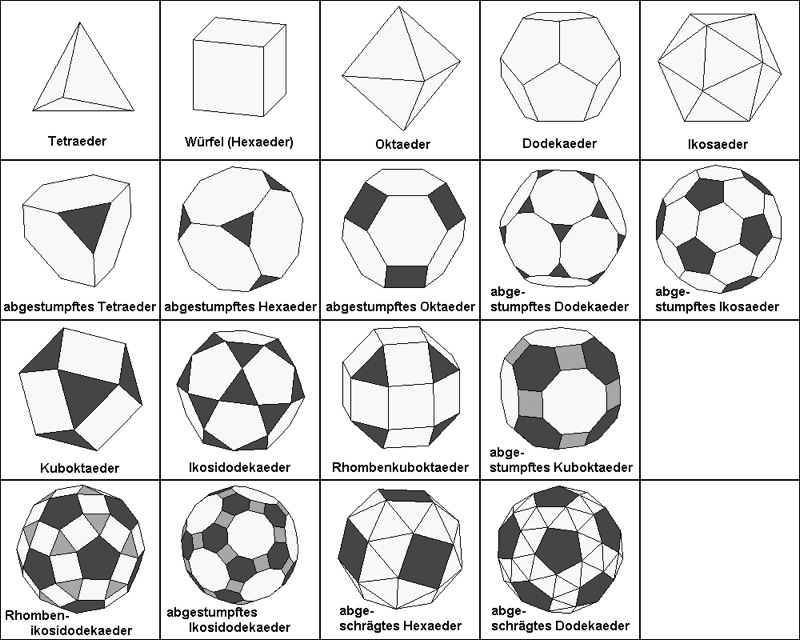
\includegraphics[width=0.8\textwidth]{pictures/polyeders}
\end{center}
\caption{Die f\"unf regelm\"assigen Polyeder mit verwandten}
\end{figure}

F\"ur den griechischen Philosophen \textsc{Plato} (427--347 v.~Chr.) waren diese f\"unf K\"orper Grundbausteine seines Weltsystems: Sie entsprachen den vier Elementen Feuer, Erde, Wasser und Luft. Das Dodekaeder entsprach einer Schale, die das ganze Universum einh\"ullt. Daher werden die f\"unf regelm\"assigen Polyeder auch \definition{platonische K\"orper} genannt.

\begin{figure}[h!]
\begin{center}
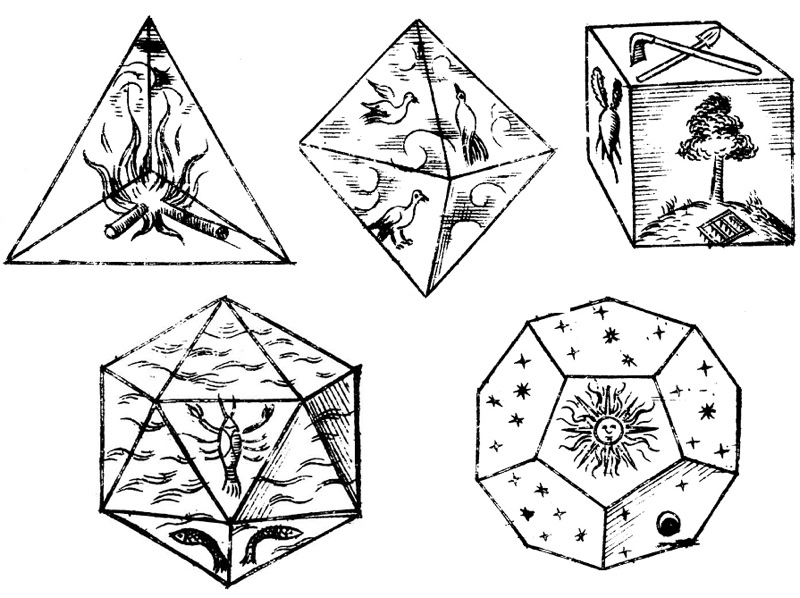
\includegraphics[width=0.382\textwidth]{pictures/platonkoerper}
\end{center}
\caption{Die f\"unf platonischen K\"orper und ihre Bedeutung als Elemente}
\end{figure}

Diese Idee Platons kann als erster bekannter Versuch interpretiert werden, die Welt mit einem Atombild zu erkl\"aren. \textsc{Platon} stellte auch Regeln auf, wie die einzelnen Elemente miteinander reagieren oder ineinander \"ubergef\"uhrt werden k\"onnen.

Selbst die Natur bevorzugt bei Kristallformen der Platon'schen Körper Gestalt.
\begin{figure}
\begin{center}
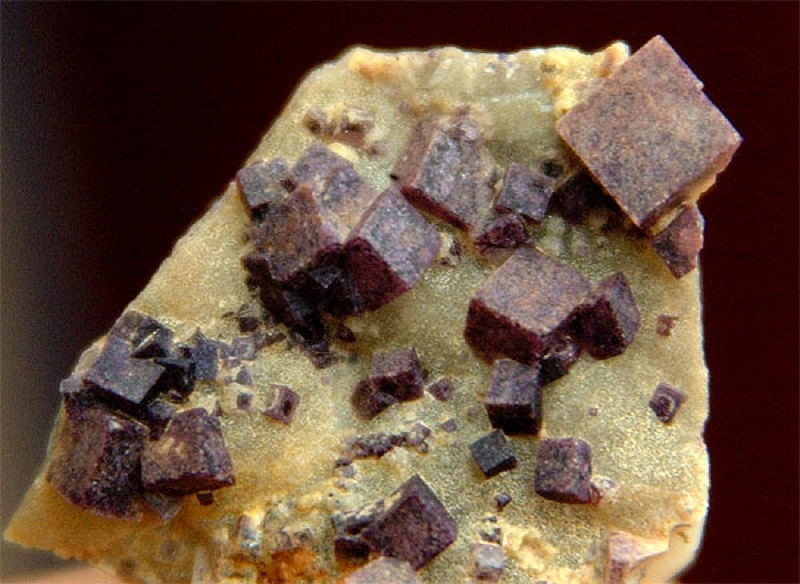
\includegraphics[width=0.382\textwidth]{pictures/kristallh}
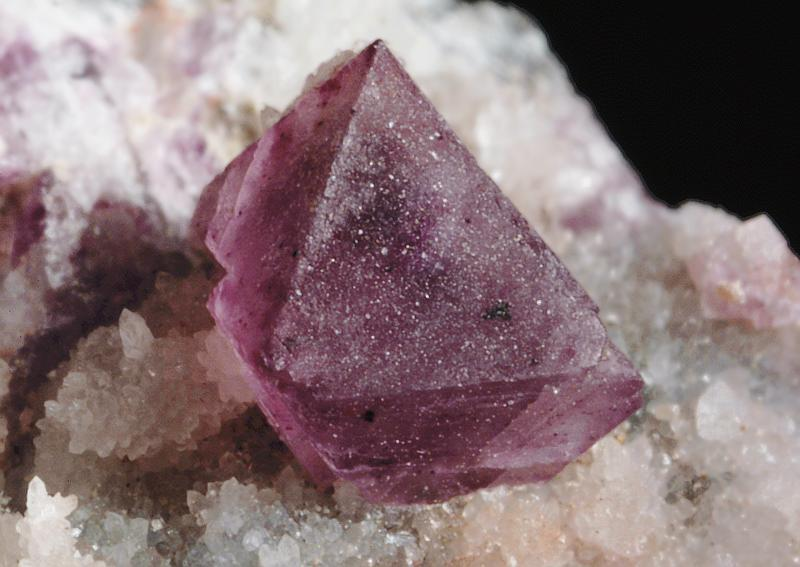
\includegraphics[width=0.382\textwidth]{pictures/kristallo}
\end{center}
\caption{Fluorkristalle (W\"urfel und Oktaeder)}
\end{figure}
Der Astronom \textsc{Johannes Kepler} (1471--1528) benutzte diese regelm\"assigen Polyeder als Modell f\"ur die Bahnen der Planeten.
\begin{figure}
\begin{center}
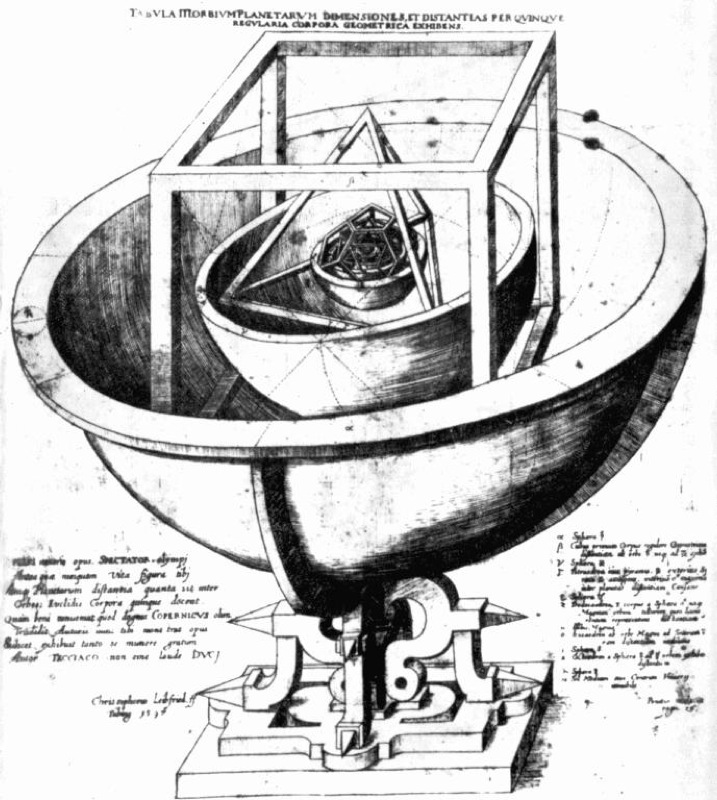
\includegraphics[width=0.618\textwidth]{pictures/kepler}
\end{center}
\caption{Planetenbahnmodell von \textsc{Kepler}}
\end{figure}
Eine der Erdbahn zugeordnete Kugel bildet den Ausgang. Ihr wird ein Dodekaeder umbeschrieben; auf dessen Umkugel liegt die Bahn des Mars. Das dieser Kugel umbeschriebene Tetraeder enth\"alt auf seiner Umkugel die Bahn des Jupiter, und der dieser Kugel umbeschriebene W\"urfel bestimmt eine Umkugel, auf der die Bahn des Saturn verl\"auft. Das der Erdbahnkugel einbeschriebene Ikosaeder tr\"agt auf seiner Inkugel die Bahn der Venus und das dieser Inkugel einbeschrieben Oktaeder enth\"alt auf seiner Inkugel die Bahn des Merkurs.

\begin{uebenv}{eminuskplusfgleichzwei}
F\"ullen Sie folgende Tabelle aus:
\begin{center}
\begin{tabular}{|c|c|c|c|}\hline
\spaltenheight\textbf{K\"orper} & \textbf{Ecken} & \textbf{Fl\"achen} & \textbf{Kanten}\spaltensep \hline
\spaltenheight Tetraeder & & & \spaltensep \hline
\spaltenheight Hexaeder & & & \spaltensep \hline
\spaltenheight Oktaeder & & & \spaltensep \hline
\spaltenheight Dodekaeder & & & \spaltensep \hline
\spaltenheight Ikosaeder & & & \spaltensep \hline
\end{tabular}
\end{center}
Fällt dir beim Betrachten der Tabelle auch auf, was \textsc{Leonard Euler} entdeckt hat?
\end{uebenv}

\subsection{Der Euler'sche Polyedersatz}

Obwohl sich die griechischen Mathematiker intensiv mit den Polyedern besch\"aftigt haben, wurde der folgende Satz erst von \textsc{Leonard Euler} (1707--1783) entdeckt.

\begin{csatz}[Euler'scher Polyedersatz]
Es sei $E$ die Anzahl Ecken, $K$ die Anzahl Kanten und $F$ die Anzahl Seitenfl\"achen eines beliebigen Polyeders. Dann gilt:
$$E-K+F=2.$$
\end{csatz}

\begin{proof}
Wir haben diesen Satz bereits bei den platonischen K\"orper best\"atigt. Die folgenden Beweisschritte werden am Beispiel eines W\"urfels demonstriert. Man stelle sich dabei vor, dass die Oberfl\"ache des Polyeders aus einer Gummihaut besteht.

\begin{minipage}{0.618\textwidth}
\begin{enumerate}
\item Nach Herausnehmen einer Fl\"ache ($F\rightarrow F-1$) kann man die Oberfl\"ache so stark deformieren, dass sie schliesslich flach in der Ebene liegt.\\
\item Triangulation: In jedem Vieleck, das nicht schon ein Dreieck ist, wird eine Diagonale eingezeichnet: ($K\rightarrow K+1, F\rightarrow F+1$) $E-K+F$ bleibt konstant.\\
\item Bei den Dreiecken, die nur eine Kante auf der Randlinie haben, wird alles entfernt, was nicht zugleich zu anderen Dreiecken geh\"ort: ($K\rightarrow K-1, F\rightarrow  F-1$) $E-K+F$ bleibt konstant.\\
\item Bei den Dreiecken, die zwei Kanten auf der Randlinie haben, wird auch alles entfernt, was nicht zugleich zu anderen Dreiecken geh\"ort: ($E\rightarrow  E-1, K\rightarrow  K-2, F\rightarrow  F-1$) $E-K+F$ bleibt konstant.\\
\item Die Punkte 3. und 4. werden so lange wiederholt, bis zuletzt nur noch ein Dreieck mit $E-K+F=1$ \"ubrig bleibt.\\
\end{enumerate}
\end{minipage}
\hspace*{2cm}
\begin{minipage}{1.7cm}
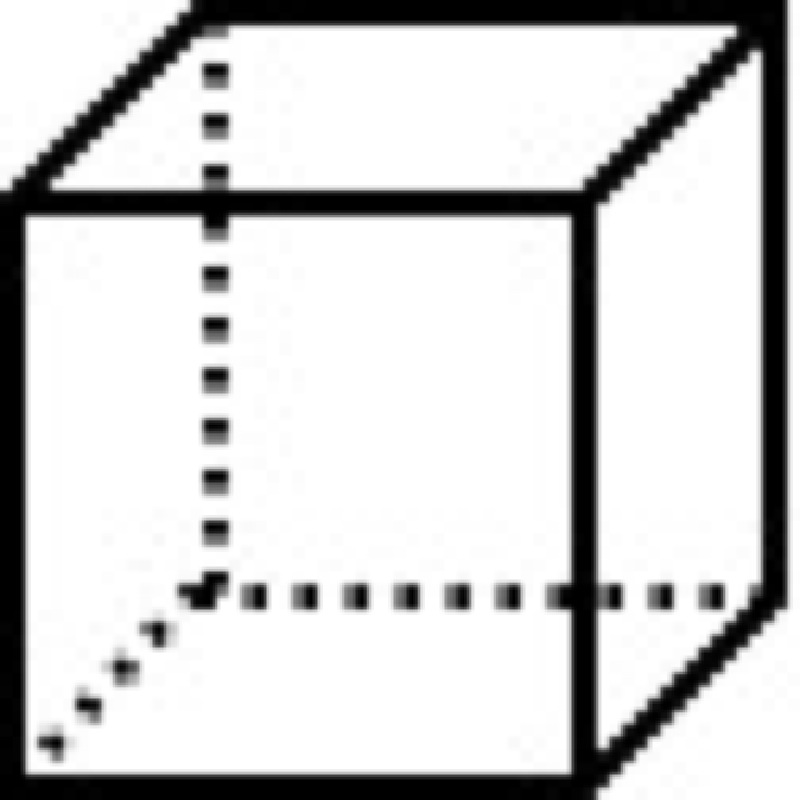
\includegraphics[width=1.7cm]{pictures/wuerf1}\\[3ex]
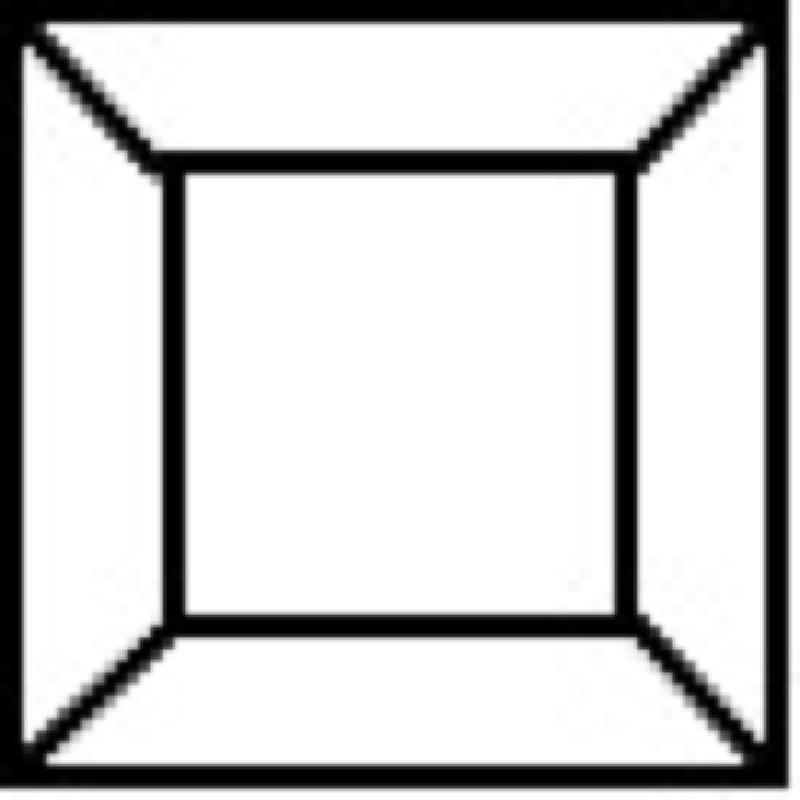
\includegraphics[width=1.7cm]{pictures/wuerf2}\\[4ex]
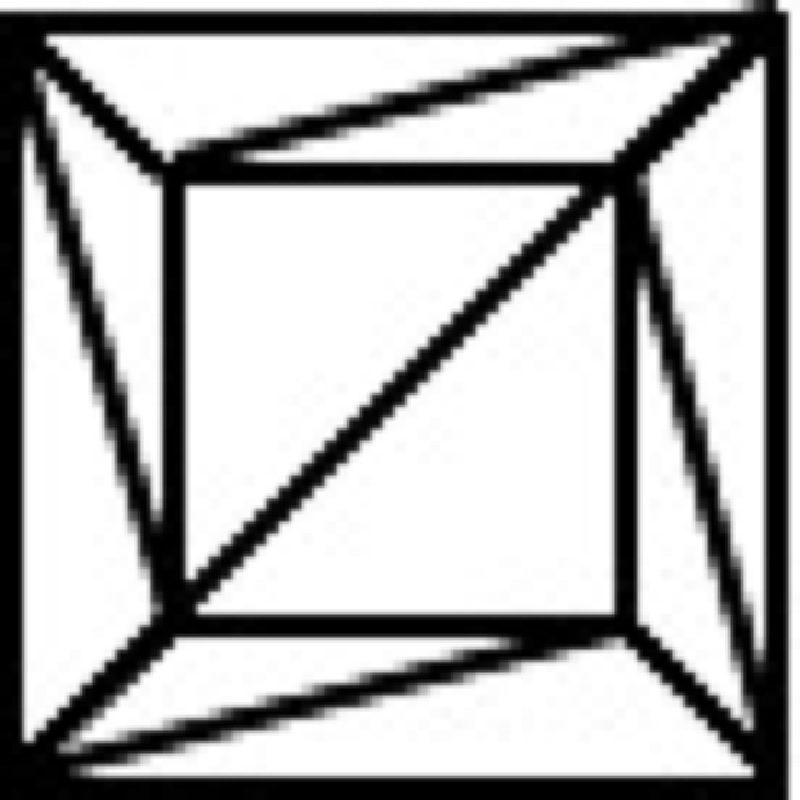
\includegraphics[width=1.7cm]{pictures/wuerf3}\\[5ex]
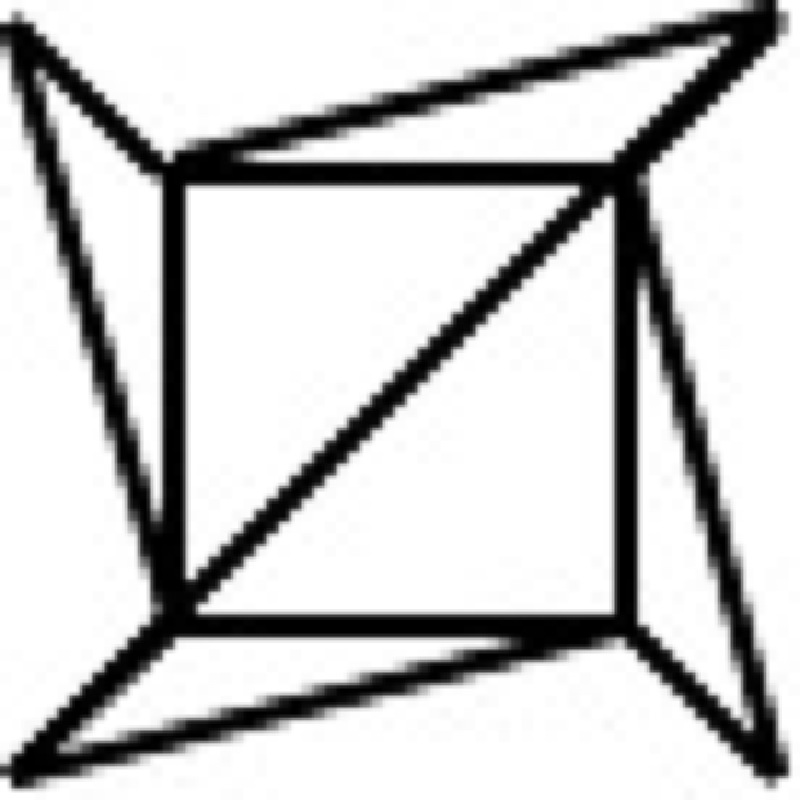
\includegraphics[width=1.7cm]{pictures/wuerf4}\\[6ex]
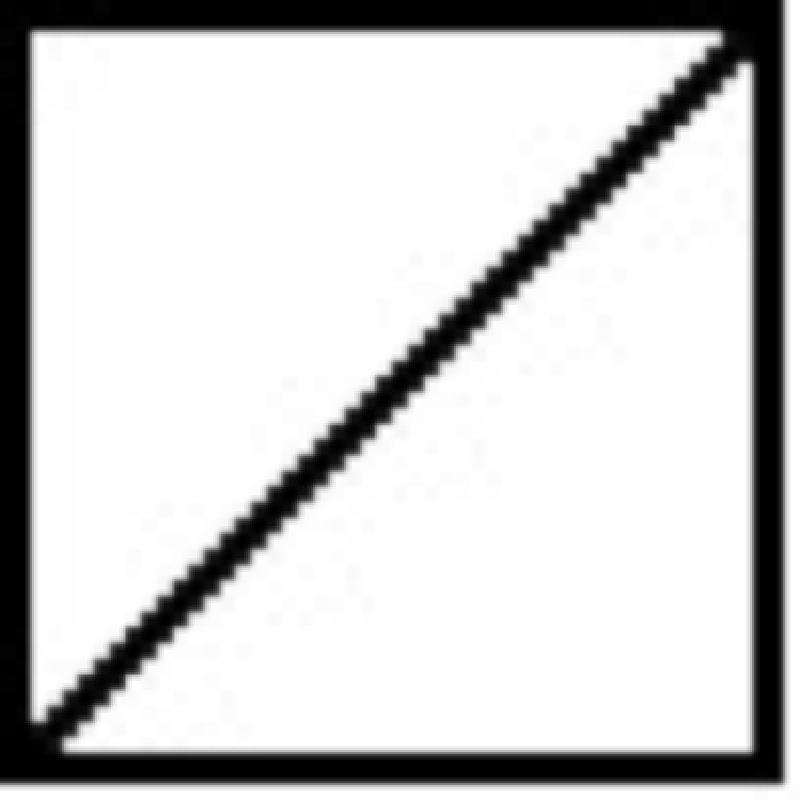
\includegraphics[width=1.7cm]{pictures/wuerf5}\\[7ex]
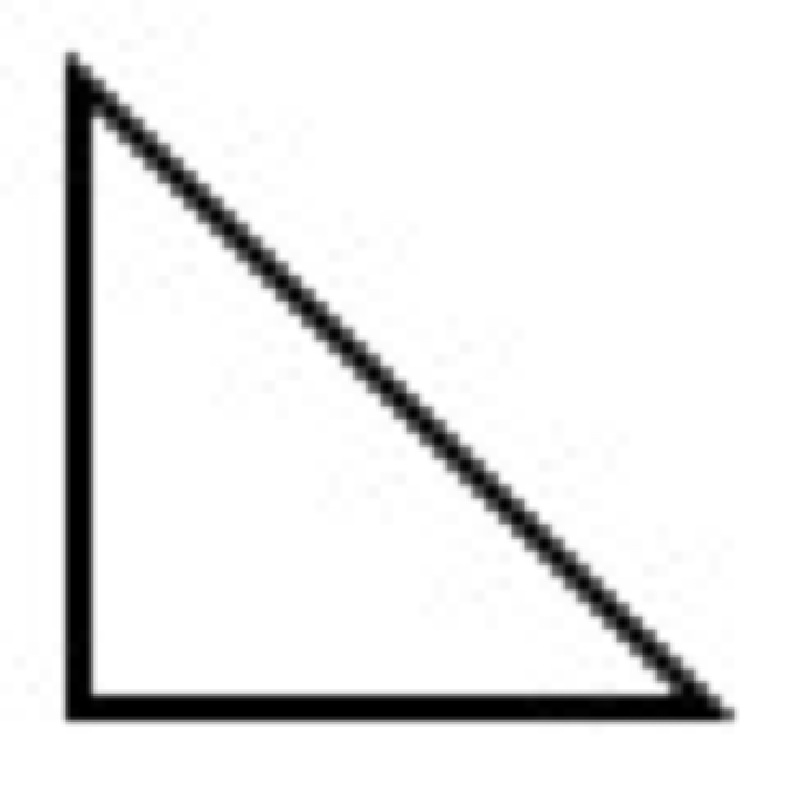
\includegraphics[width=1.7cm]{pictures/wuerf6}
\end{minipage}\\
Bei diesen Operationen hat sich der Wert von $E-K+F=1$ nicht ver\"andert. Ber\"ucksichtigt man noch Punkt 1., so muss f\"ur das Polyeder $E-K+F=2$ gelten.
\end{proof}


\begin{uebenv}
Ein konvexes Polyeder hat 14 Fl\"achen und 24 Ecken. Wie viele Kanten hat es?
\end{uebenv}

\clearpage

\subsection{Notizen zu den Übungen}

\begin{lsg}{anzahlpolyeder}
Der Innenwinkel an einer Ecke eines gleichseitigen Dreiecks ist $60^\circ$. Man kann daher nicht mehr als $5$ solche in einer Ecke zusammenkommen lassen, da sonst die Winkelsumme $360^\circ$ oder mehr beträgt, der Polyeder also nicht mehr konvex ist (es zwingt ihn in die Ebene oder konkav). Das gleiche Argument gilt für die Quadrate ($90^\circ$) und die regelmässigen Fünfecke ($108^\circ$). Man sieht so zudem, dass nicht mehr als zwei reguläre Sechsecke ($120^\circ$) an einer Ecke zusammenkommen könnten, um konvex zu bleiben.
\end{lsg}
\begin{lsg}{eminuskplusfgleichzwei}
    \begin{center}
\begin{tabular}{|c|c|c|c|}\hline
\spaltenheight\textbf{K\"orper} & \textbf{Ecken} & \textbf{Fl\"achen} & \textbf{Kanten}\spaltensep \hline
\spaltenheight Tetraeder & 4 & 4 & 6\spaltensep \hline
\spaltenheight Hexaeder & 8 & 12 & 6\spaltensep \hline
\spaltenheight Oktaeder & 6 & 12 & 8\spaltensep \hline
\spaltenheight Dodekaeder & 20 & 30 & 12\spaltensep \hline
\spaltenheight Ikosaeder & 12 & 30 & 20\spaltensep \hline
\end{tabular}
\end{center}
\end{lsg}
\begin{lsg}
Es ist nach Euler'schem Polyedersatz $24-K+14=2$, also hat es $36$ Kanten.
\end{lsg}

\clearpage

\section{Polarkoordinaten}

In einem rechtwinkligen Koordinatensystem kann die Lage eines Punktes $P\neq(0|0)$ nicht nur durch seine kartesischen Koordinaten $(x|y)$, sondern auch durch seinen Abstand $r>0$ vom Ursprung und einem Richtungswinkel $\varphi\in[0,2\pi)$ eindeutig angegeben werden.

<<<<<<< Updated upstream
\begin{center}\definecolor{qqwuqq}{rgb}{0,0.39,0}
=======
\begin{center}
>>>>>>> Stashed changes
\scalebox{1.1}{
\begin{tikzpicture}[line cap=round,line join=round,>=triangle 45,x=0.5cm,y=0.5cm]
\draw[->,color=black] (-2.78,0) -- (10,0);
\foreach \x in {-2,-1,1,2,3,4,5,6,7,8,9}
\draw[shift={(\x,0)},color=black] (0pt,2pt) -- (0pt,-2pt);
\draw[color=black] (9.66,0.08) node [anchor=south west] {$x$};
\draw[->,color=black] (0,-2.28) -- (0,8.3);
\foreach \y in {-2,-1,1,2,3,4,5,6,7,8}
\draw[shift={(0,\y)},color=black] (2pt,0pt) -- (-2pt,0pt);
\draw[color=black] (0.1,7.9) node [anchor=west] {$y$};
\clip(-2.78,-2.28) rectangle (10,8.3);
<<<<<<< Updated upstream
\draw [shift={(0,0)},line width=1.6pt,color=qqwuqq,fill=qqwuqq,fill opacity=0.1] (0,0) -- (0:2) arc (0:44.22:2) -- cycle;
=======
\draw [shift={(0,0)},line width=1.6pt,color=ForestGreen,fill=ForestGreen,fill opacity=0.1] (0,0) -- (0:2) arc (0:44.22:2) -- cycle;
>>>>>>> Stashed changes
\draw [line width=1.5pt] (5.92,5.76)-- (0,0);
\fill [color=black] (5.92,5.76) circle (1.5pt);
\draw[color=black] (6.2,6.2) node {$P$};
\draw[color=black] (2.76,3.26) node {$r$};
<<<<<<< Updated upstream
\draw[color=qqwuqq] (1.26,0.5) node {$\varphi$};
=======
\draw[color=ForestGreen] (1.26,0.5) node {$\varphi$};
>>>>>>> Stashed changes
\end{tikzpicture}
}
\end{center}

\begin{cdef}[Polarkoordinaten]
Das Paar $(r|\varphi)$ nennt man die \emph{Polarkoordinaten} von $P$.
\end{cdef}

Polarkoordinaten können insbesondere dann nützlich sein, wenn man in Kugelsymmetrien rechnet oder einfach punktsymmetrische Probleme lösen muss.

\clearpage
\listoffigures
%\listoftables
%\newpage
%\nocite{*}
%\bibliographystyle{plain}
%\bibliography{preamble/literaturgoogle}
\end{document}